\documentclass[a4paper,12pt]{report}
\usepackage[T2A]{fontenc}
\usepackage[utf8]{inputenc}
%\usepackage[14pt]{extsizes}
\usepackage[english,russian]{babel}
\usepackage {titlesec, textcase} 
\usepackage{amssymb,amsfonts,amsmath,cite,enumerate,float}
\usepackage[dvips]{graphicx}
\usepackage {indentfirst}
\usepackage{pscyr}
\usepackage{cite,enumerate}

% поддержка гиперссылок; гиперссылки в pdf, должен быть последним загруженным пакетом
\ifx\pdfoutput\undefined
    \usepackage[unicode,dvips]{hyperref}
\else
    \usepackage[pdftex,colorlinks,unicode,bookmarks]{hyperref}
\fi

%\makeatletter
%\titleformat{\chapter}{\huge\bfseries}{\thechapter. }{0pt}{\huge} % Правим названия глав
%\bibliographystyle{utf8gost71u} % Оформляем библиографию по ГОСТ 7.1 (ГОСТ Р 7.0.11-2011, 5.6.7)
%\renewcommand{\@biblabel}[1]{#1.} % Заменяем библиографию с квадратных скобок на точку
%\makeatother

\makeatletter
%\titleformat{\chapter}{\huge\bfseries}{\thechapter. }{0pt}{\huge} % Правим названия глав
\bibliographystyle{IEEEtran} % Оформляем библиографию по ГОСТ 7.1 (ГОСТ Р 7.0.11-2011, 5.6.7)
\renewcommand{\@biblabel}[1]{#1.} % Заменяем библиографию с квадратных скобок на точку
\makeatother

\linespread{1.3} % Полуторный интвервал (ГОСТ Р 7.0.11-2011, 5.3.6)
\sloppy % Избавляемся от переполнений
\clubpenalty=10000 % Запрещаем разрыв страницы после первой строки абзаца
\widowpenalty=10000 % Запрещаем разрыв страницы после последней строки абзаца
\makeatletter
\renewcommand{\@biblabel}[1]{#1.} % Заменяем библиографию с квадратных скобок на точку:
\makeatother

% Меняем поля страницы
\usepackage{geometry}
\geometry{left=3cm}
\geometry{right=1.5cm}
\geometry{top=2cm}
\geometry{bottom=2cm}

% Меняем везде перечисления на цифра.цифра
\renewcommand{\theenumi}{\arabic{enumi}}
\renewcommand{\labelenumi}{\arabic{enumi}}
\renewcommand{\theenumii}{.\arabic{enumii}}
\renewcommand{\labelenumii}{\arabic{enumi}.\arabic{enumii}.}
\renewcommand{\theenumiii}{.\arabic{enumiii}}
\renewcommand{\labelenumiii}{\arabic{enumi}.\arabic{enumii}.\arabic{enumiii}.}
\renewcommand{\contentsname}{Содержание}
\renewcommand{\bibname}{Список использованных источников}


\newcommand{\angstrom}{\text{\normalfont\AA}}

%\makeatletter
%\titleformat{\chapter}{\huge\bfseries}{\thechapter. }{0pt}{\huge}
%\makeatother

\addto\captionsrussian{
	\renewcommand{\contentsname}{Оглавление} % (ГОСТ Р 7.0.11-2011, 4)
	\renewcommand{\appendixname}{Приложение} % (ГОСТ Р 7.0.11-2011, 5.7)
	\renewcommand{\bibname}{Список литературы} % (ГОСТ Р 7.0.11-2011, 4)
}


\graphicspath{{images/}}

\begin{document}

\begin{titlepage}
\newpage
\begin{center}
Министерство образования и науки Российской Федерации\\
\vspace{1em} 
Федеральное государственное автономное образовательное учреждение\\
высшего профессионального образования\\
<<Московский физико-технический институт\\
(государственный университет)>>\\
\vspace{1em}
Факультет проблем физики и энергетики\\
\vspace{1em}
Кафедра нелинейных и динамических процессов в астрофизике и геофизике\\
\vspace{5em}
\textbf{\large\MakeTextUppercase{Подготовка программы наблюдений космической миссии "Спектр-УФ": отбор кандидатов в звёзды типа Т Тельца в созвездии Змеи}}\\
\vspace{1em}
Выпускная квалификационная работа\\
(бакалаврская работа)\\
\vspace{1em}
Направление подготовки 03.03.01 Прикладные математика и физика\\
\end{center}
\begin{flushleft}
\vspace{3em}
Выполнила:\\
студентка 183 группы \hrulefill Молярова Тамара Сергеевна\\
\vspace{3em}
Научный руководитель:\\
д.ф.-м.н., ведущий научный сотрудник \hrulefill Сачков Михаил Евгеньевич\\
\vspace{\fill}
\end{flushleft}
\begin{center}
Москва 2015
\end{center}
\end{titlepage}

\tableofcontents

\chapter{Введение}


\section{T Tauri звёзды}
Целью данной работы является поиск звёзд, относящихся к определённому классу: звёзд типа Т Тельца. 
Это предшественники звёзд, подобных Солнцу, а также планетарных систем. Поэтому их изучение очень важно для понимания процесса формирования Солнечной системы, её эволюции и образования планет. 

Как молодые звёзды, звёзды типа Т Тельца обнаруживаются в областях звездообразования. Т Тельца, по имени которой назван этот класс звёзд, расположена в 

\section{Изучаемая область}

В данной работе изучается тёмная туманность, находящаяся в созвездии Змея и Орёл (Serpens-Aquila Rift). Межзвёздная среда в ней находится в холодной фазе, то есть состоит из плотных и холодных облаков газа, в основном молекулярного водорода H$_{2}$. Именно из такого вещества формируются звёзды. Существуют исследования, подтверждающие, что в этой туманности происходит активное звездообразование [Far-ultraviolet Observation of the Aquila Rift with FIMS SPEAR].

\begin{figure}[h]
\center{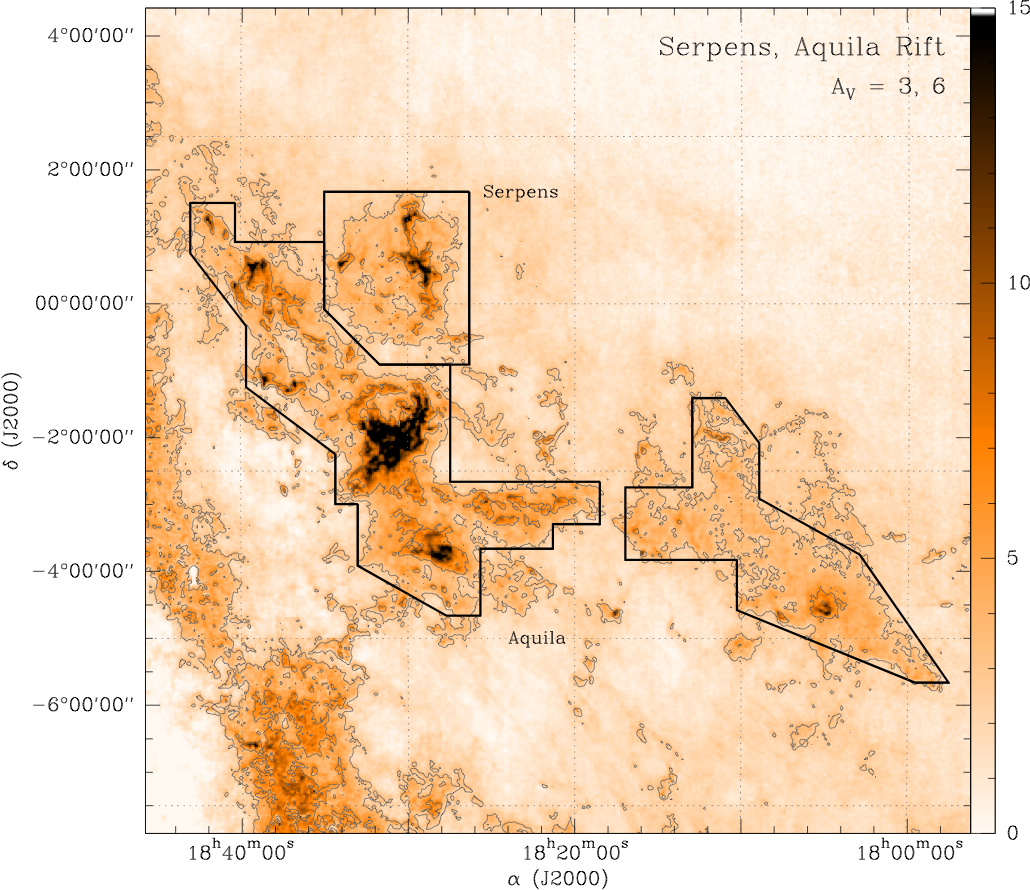
\includegraphics[width=0.6\linewidth]{gb_serpens.jpg}}
\hfill
\caption{Туманность в созвездии Змея, изображение от космического телескопа Гершель (Hershel)}
\label{fig:area}
\end{figure}


Расстояние до туманности оценивается по-разному. Та её часть, которая относится к созвездию Орёл, расположена на расстоянии 225$\pm$55 парсек от Земли. Область, относящаяся к Змее, несколько дальше. Согласно измерениям параллакса, проведённым на радиоинтерферометре VLBA, она находится на расстоянии 415$\pm$25 парсек[ссылка та же].

Несмотря на то, что исследуемая область известна наличием звездообразования, ни одна звезда в ней не идентифицирована как относящаяся к типу Т Тельца. Это связано с расположением туманности близко к галактической плоскости и недостатком наблюдений в нужных спектральных диапазонах.

Мы рассматривали область неба, для которой прямое восхождение лежит в интервале от 17.96 до 18.72, а наклонение от -5 до 5.5. Вторая часть туманности не рассматривалась из-за отсутствия необходимых наблюдений.

\section{Метод поиска}

По фотометриям galex, цветовым диаграммам + отсев по собственным движениям, эффективным температурам и simbad.

\section{Актуальность}

О космическом телескопе Спектр-УФ. Неисследованная область

\chapter{T Tauri звёзды}

\section{Звёзды типа Т Тельца}
Звёзды типа Т Тельца - это маломассивные молодые звёзды, находящиеся на пути к главной последовательности. Обычно они находятся недалеко от отражательных или тёмных туманностей, оставшихся от газопылевого облака, из которого эти звёзды сформировались. Эти звёзды находятся в той части диаграммы Герцшпрунга - Рассела, которая соответствует звёздам с массами около 2-3 солнечных. С точки зрения звёздной эволюции они находятся в стадии гравитационного сжатия и, как молодые объекты, имеют близкую к солнечной металличность \cite{dod2013}. Характерными чертами также является избыточная эмиссия в ИК и УФ дапазонах.

Выделяют два подтипа этих звёзд: классические звёзды типа Т Тельца (classical T Tauri stars, CTTS) и звёзды типа Т Тельца со слабыми линиями (weak-lined T Tauri stars). Звёзды обоих подтипов находятся на одной стадии эволюции, имеют малую массу, и их металличность близка к солнечной. Различие состоит в том, что в спектрах классических звёзд типа Т Тельца присутствуют сильные эмиссионные линии, указывающие на то, что эти звёзды проявляют определённого рода активность. У звёзд типа Т Тельца со слабыми линиями эмиссионные линии гораздо слабее. Граница между подтипами проводится по эквивалентной ширине линии H$\alpha$. 

%%%%%%%%%%%%%%%%%%%%%%%%%%%%%%%%%%%%%%%%%%%%%%%%%%%%%%%%%%%%%%%%%%%%%%%%%%%%%%%%%%%%%%%%%

\section{Спектральные особенности}
Звёзды типа Т Тельца относятся к классу переменных звёзд. Первоначально они были выделены в отдельный класс на основе чисто спектроскопических характеристик: наличия эмиссии в линиях H$\alpha$ и Fe I, а также класс светимости IV-V. 

Сейчас выделяются следующие критерии принадлежности к типу \cite{dod2013}:
\begin{itemize}
	\item Наличие поблизости тёмной или отражательной туманности;
	\item	Спектральный класс F5-M, класс светимости IV-V;
	\item	Эмиссия в линиях H и He I, а также нейтральных и однократно ионизированных металлов;
	\item	Сильная линия поглощения Li I 6707 A;
\end{itemize}

Присутствие линии Li указывает на молодость звёзд, так как согласно теоретическим расчётам литий быстро выгорает.

Эмиссионный спектр CTTS напоминает спектр солнечной хромосферы. Поэтому изначально считалось, что для них характерна высокая хромосферная активность \cite{krav2004}. Но ожидаемое в этой модели сильное рентгеновское излучение не нашло экспериментального подтверждения.

В настоящее время считается, что спектральные особенности CTTS обусловлены наличием аккреционного диска. Если также предположить наличие магнитного поля, направление которого не совпадает с осью вращения звезды, то удаётся объяснить асимметричность эмиссионных линий. Предполагается, что они образуются на границе магнитосферы. Также аккреция вещества на звезду вызывает возникновение джетов. Это биполярные узконаправленные струи газа, истекающие со звезды. Они наблюдаются обычно в запрещённых линиях [SiI], [OI].

Наличие протопланетных дисков и магнитного поля у многих звёзд типа Т Тельца подтверждается наблюдениями.

Чтобы отличить звёзды типа Т Тельца от других, нам нужно знать характеристики их спектров, в особенности те из них, которые можно наблюдать в фотометриях. Как следствие существования аккреционного диска и истечения вещества на звезду, у TTS наблюдается избыток излучения в различных спектральных диапазонах, а именно:
\begin{itemize}
	\item Избыток в инфракрасном диапазоне вплоть до миллиметровых длин волн, обусловленный как собственным излучением нагретого диска, так и переизлучением поглощённого им излучения звезды и джетов.
	\item Избыток в оптическом диапазоне – свечение плазмы, нагретой до температуры 7000-10000 K. Это так называемое вуалирование -- континуальное излучение нефотосферной природы. 
	\item Избыток в ультрафиолетовом диапазоне -- свечение плазмы с температурой электронов от 10000 K до 50000 K, причём присутствует как излучение в континууме, так и различные эмиссионные линии: нейтральные атомы (H I, O I, C I), однократно (C II, Si II, Fe II, Mg II, O I) и многократно (C IV, N V, O VI) ионизованные атомы, молекулярный водород.
	\item Избыток в рентгеновском диапазоне, вызванный высокой активностью магнитосферы звезды, свечением короны и ударными волнами в аккреционном диске.
\end{itemize}

%кортинка спектра T Tauri

%%%%%%%%%%%%%%%%%%%%%%%%%%%%%%%%%%%%%%%%%%%%%%%%%%%%%%%%%%%%%%%%%%%%%%%%%%%

\section{Методы поиска}
 Изначально главными критериями поиска были лишь самые основные характеристики звёзд типа Т Тельца, как-то: близость к молекулярным облакам, избыток в инфракрасном диапазоне, присутствие магнитного поля. Позже, с появлением широкомасштабных обзоров неба, стали учитываться эквивалентная ширина линии H $\alpha$, собственные движения звёзд и избыток излучения в рентгеновском диапазоне. Также могут быть использованы оптические и инфракрасные данные и распределение спектральной энергии (SED) в этих диапазонах, в которых можно выделить черты, характерные для аккреционных дисков. Однако этими методами труднее обнаружить WTTS. Единственным действительно надёжным критерием является присутствие линии Li, как показатель молодости звезды.

Несмотря на то, что у звёзд типа Т Тельца присутствует существенный ультрафиолетовый избыток, большинство исследований, направленных на их поиск, проводилось в инфракрасном и рентгеновском диапазонах. С появлением ультрафиолетового обзора неба от миссии GALEX есть возможность использования и 





\chapter{Данные}
Для поиска кандидатов применялись данные, взятые из трёх каталогов точечных источников. За основу брался список всех источников, относящихся к рассматриваемой области, которые пронаблюдал телескоп GALEX.
Для этого списка проводилась кросс-идентификация с каталогами 2MASS и UCAC4 с целью получения данных о звёздных величинах в фильтрах инфракрасного и видимого диапазонов. 

%%%%%%%%%%%%%%%%%%%%%%%%%%%%%%%%%%%%%%%%%%%%%%%%%%%%%%%%%%%%%%%%%%%%%%%%%%%%%%%%%%%%%%%%

\section{GALEX}
GALEX (Galaxy Evolution Explorer) -- это ультрафиолетовый обзорный космический телескоп с полуметровым зеркалом, запущенный в 2003 году. Его целью является исследование эволюции звездообразования в галактиках от ранней вселенной до наших дней. Так как наблюдения в ультрафиолете недоступны с Земли, его каталог точечных источников является единственным источником данных в этом спектральном диапазоне.

Обзор неба от GALEX состоит из круглых изображений радиусом 0.7 градусов и покрывает две трети небесной сферы. Наблюдения проводились в двух фильтрах: FUV(Far Ultraviolet), охватывающий диапазон 125-180 нм, и NUV(Near Ultraviolet) в диапазоне 170-300 нм с пространственным разрешением 4.3 и 5.3 угловых секунд соответственно.

%%кортинка с фильтерами и со спектром в фильтре

Телескоп избегал наблюдений вблизи галактической плоскости и Магеллановых облаков, а также ярких звёзд, так как это могло привести к перегоранию чувствительных детекторов. Минимальная допустимая звёздная величина равна 9.5 и 8.9 для FUV и NUV соответственно. Максимальная звёздная величина составляет 22.3. Из-за высокой чувствительности телескопа в каталоге присутствует много ложных объектов, случайных шумов, которые были приняты за реальные источники. В дальнейшем эти паразитные источники отсеются при кросс-идентификации, не найдя соответствий в других спектральных диапазонах.

Так как интересующий нас участок неба находится близко к галактической плоскости, он не полностью покрыт наблюдениями. Для левой части туманности данных нет, а правая покрыта наблюдениями на 70\%.

%%кортика с покрытием

Для выбранной области нашлось 2968 источников, причём для некоторых из них отсутствовала звёздная величина в фильтре FUV. Их пришлось отбросить, так как эта информация существенна для нашего исследования.

%%%%%%%%%%%%%%%%%%%%%%%%%%%%%%%%%%%%%%%%%%%%%%%%%%%%%%%%%%%%%%%%%%%%%%%%%%%%%%%%%%%%%%%%%%%%%%%%%

\section{Кросс-идентификация с 2MASS и UCAC4}
После получения исходного списка источников он был кросс-идентифицирован с каталогами 2MASS и UCAC4. То есть для каждого источника из списка мы искали соответствие в другом каталоге, основываясь на равенстве или близости их координат. Параметр кросс-корреляции взят равным 3 угловым секундам. Это максимальное расстояние между источниками из разных каталогов, при котором они будут считаться одним источником.

2MASS(Two Micron All-Sky Survey) -- это полный обзор всего неба на длинах волн около 2 микрон. Он содержит информацию о звёздных величинах в фильтрах J, H и Ks с длинами волн 1.25, 1.65 и 2.17 мкм соответственно.

Так как  этот обзор создавался с помощью больших наземных телескопов, пространственное разрешение здесь гораздо выше, чем у GALEX, и источники можно считать действительно точечными. Из-за низкой точности GALEX объекты в нём размазаны и эффективно имеют радиус около 2.2-2.7 угловых секунд. Поэтому при кросс-идентификации объект из GALEX считается совпавшим с объектом из 2MASS, если он попадает внутрь окружности с радиусом 3 угловых секунды.

Все источники из первоначального списка, не идентифицированные в каталоге 2MASS, должны быть сочтены ложными и откинуты.

Каталог UCAC4 содержит данные в фильтрах видимого диапазона: V и B фотометрической системы Джонсона, а также i и r фотометрической системы SDSS. Кроме того, из него мы берём информацию о собственных движениях звёзд. В него включены только звёзды. Их величины лежат в интервале от 8 до 16, ярче, чем в GALEX. Поэтому те объекты из списка, которые не нашли соответствия в UCAC4, не должны отбрасываться.

Инфракрасные звёздные величины необходимы нам для построения диаграмм цвет-цвет и формулирования критериев поиска звёзд типа Т Тельца. Величины в видимом диапазоне используются для иллюстрации на цветовых диаграммах и для дополнительного критерия. Также они нужны для оценки эффективных температур.

После кросс-идентификации список сократился до 726 объектов.

\section{Используемые инструменты}
casjobs для получения данных с галекса. visier для кросс-матчинга. aladin для картинок



\chapter{Отбор}
Основной этап поиска кандидатов -- это отбор звёзд, соответствующих нижеизложенным критериям. Для этого необходимо наличие информации лишь о звёздной величине кандидатов в ультрафиолетовом и инфракрасном спектральных диапазонах, а спектральные данные не требуются.

При создании критериев мы будем придерживаться следующей модели. Взяв за образец выборку известных звёзд типа Т Тельца, находящихся на небольшом расстоянии, мы определим положение этих звёзд на цветовых диаграммах. Все источники, попавшие в ту же область диаграммы цвет-цвет, мы сочтём первичными кандидатами, определив условные границы этой области.

В основе данной модели составления критериев лежит работа Гомез де Кастро 2014 \cite{AIGdC2014galex}, в которой аналогичное исследование проводится для молекулярного облака Тельца.

\section{Эталонная выборка}
Чтобы определить, какого поведения мы ожидаем от кандидатов в T Tauri звёзды, нам понадобится образцовая выборка, состоящая из известных и подтверждённых T Tauri звёзд. Их названия и фотометрические данные приведены в \ref{tabular:etalon}.

Мы взяли звёзды, наблюдавшиеся телескопом IUE (International Ultraviolet Explorer). Выборка из 21 звезды получена в работе \cite{de1997accretion}. Далее их IUE спектры были умножены на функцию пропускания фильтров \cite{AIGdC2014galex}.

$$NUV = -2.5\times\log\left(\frac{FluxNUV}{2.06\times10^{-16}\text{erg }\text{s}^{-1}\text{cm}^{-2}\angstrom^{-1}}\right) + 20.08$$

$$FUV = -2.5\times\log\left(\frac{FluxFUV}{1.40\times10^{-15}\text{erg }\text{s}^{-1}\text{cm}^{-2}\angstrom^{-1}}\right) + 18.82$$
\vspace{1em}

\begin{table}[ht]
\caption{Эталонная выборка звёзд, используемых как образец для формулирования критериев.}
\label{tabular:etalon}
\begin{center}
\begin{tabular}{cccccccccc}
Star & Spectral & d & FUV & NUV & R & J & H & K \\
 &  type & pc & AB mag & AB  mag & mag & mag & mag & mag \\
WY Ari & K5 Bin & 275 & 17.36 & 15.26 & 12.40 & 10.229 & 9.418 & 8.901 \\
BP Tau & K7 & 140 & 17.66 & 15.97 & 11.62 & 9.10 & 8.22 & 7.736 \\
DE Tau & M2 & 140 & 17.96 & 16.49 & 11.93 & 9.18 & 8.273 & 7.799 \\
RY Tau & K1 & 140 & 17.73 & 15.38 & 9.67 & 7.16 & 6.13 & 5.395 \\
T Tau & K0 & 140 & 16.42 & 14.97 & 9.80 & 7.24 & 6.237 & 5.325 \\
DF Tau & M0-1 & 140 & 17.58 & 16.78 & 11.50 & 8.17 & 7.256 & 6.734 \\
DR Tau & K4 & 140 & 16.95 & 14.87 & 12.19 & 8.85 & 7.8 & 6.874 \\
GM Aur & K3 & 140 & 17.57 & 16.39 & 11.22 & 9.34 & 8.603 & 8.283 \\
SU Aur & G2 & 140 & 18.04 & 15.21 & 9.17 & 7.20 & 6.558 & 5.99 \\
RW Aur & K1 & 140 & 16.51 & 14.13 & 9.95 & 8.38 & 7.621 & 7.02 \\
GW Ori & G5 & 450 & 17.44 & 15.02 & 9.52 & 7.70 & 7.103 & 6.59 \\
CV Cha & G8 & 175 & 17.32 & 14.94 & 10.51 & 8.29 & 7.46 & 6.845 \\
RU Lup & K7 & 140 & 15.85 & 13.41 & 9.99 & 8.73 & 7.824 & 7.138 \\
AK Sco & F5 SB & 145 & 17.15 & 14.01 & 9.20 & 7.68 & 7.06 & 6.503 \\
DI Cep & G8 & 244 & 17.51 & 15.11 & 10.49 & 9.30 & 8.572 & 7.952 \\
HD 283572 & G5 & 140 & 18.75 & 14.77 & 9.14 & 7.41 & 7.008 & 6.869 \\
AB Dor & K0 & 15 & 16.32 & 12.8 & 6.50 & 5.32 & 4.845 & 4.686 \\
TW Hya & K7 & 56 & 15.65 & 14 & 10.19 & 8.22 & 7.558 & 7.297 \\
V2398 Oph & G8 & 125 & 16.23 & 14.48 & 10.10 & 8.62 & 7.81 & 7.23 \\
V4046 Sgr & K5.6 SB & 83 & 16.6 & 16.05 & 9.67 & 8.07 & 7.435 & 7.249 \\
FK Ser & K7 Bin & 350 & 17.72 & 16.19 & 9.41 & 7.64 & 6.92 & 6.624 \\
\end{tabular}
\end{center}
\end{table}

В эталонной выборке содержится мало WTTS и звёзд M типа, что обусловлено низкой чувствительностью телескопа IUE. Можно заметить, что в FUV звёздная величина мала, это делает более трудным поиск звёзд типа Т Тельца со слабыми линиями.

\section{Двухцветные диаграммы}
Перейдём к построению двухцветных диаграмм. Мы используем четыре типа этих диаграмм: FUV-NUV vs J-K, FUV-NUV vs H-K, NUV-H vs J-K и NUV-R vs J-K. Первые три существенны для отделения кандидатов, четвёртый же выполняет иллюстративную функцию, так как на диаграмму этого типа, требующую наличия блеска в фильтре R, попадает гораздо меньше звёзд.

\begin{figure}[ht]
\begin{minipage}[ht]{0.49\linewidth}
\center{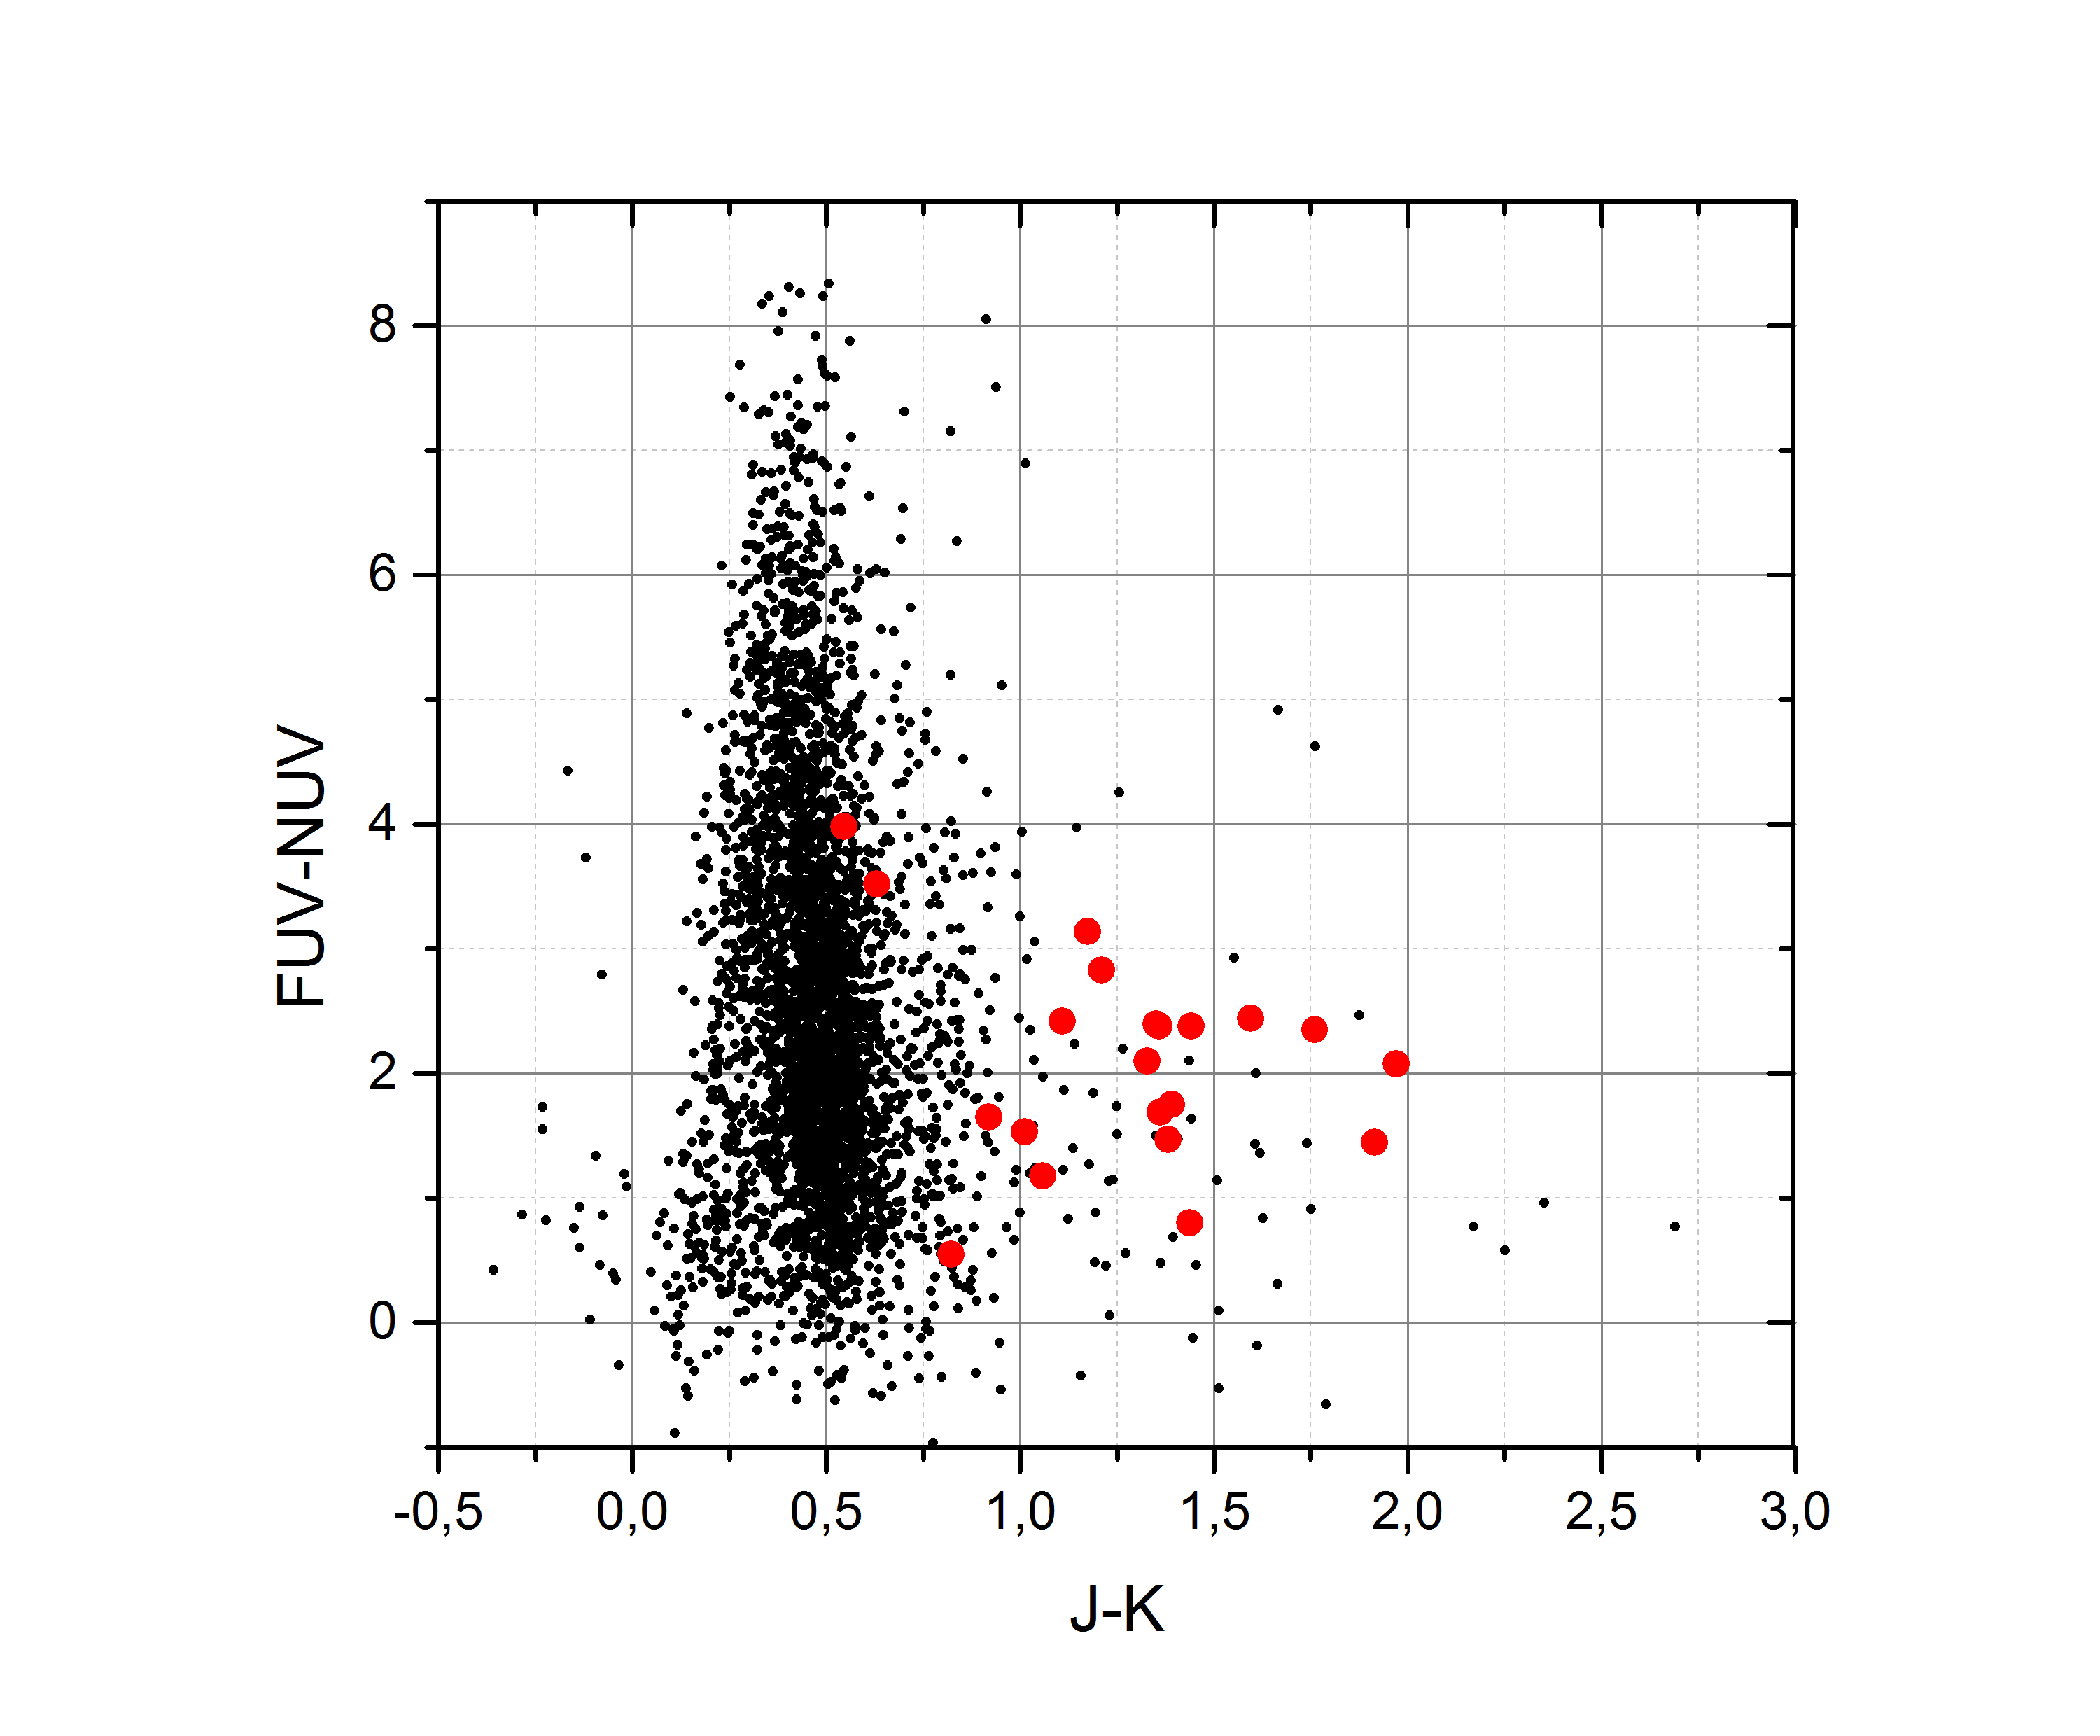
\includegraphics[width=1\linewidth]{Graph1.png} \\ FUV-NUV vs J-K}
\end{minipage}
\hfill
\begin{minipage}[ht]{0.49\linewidth}
\center{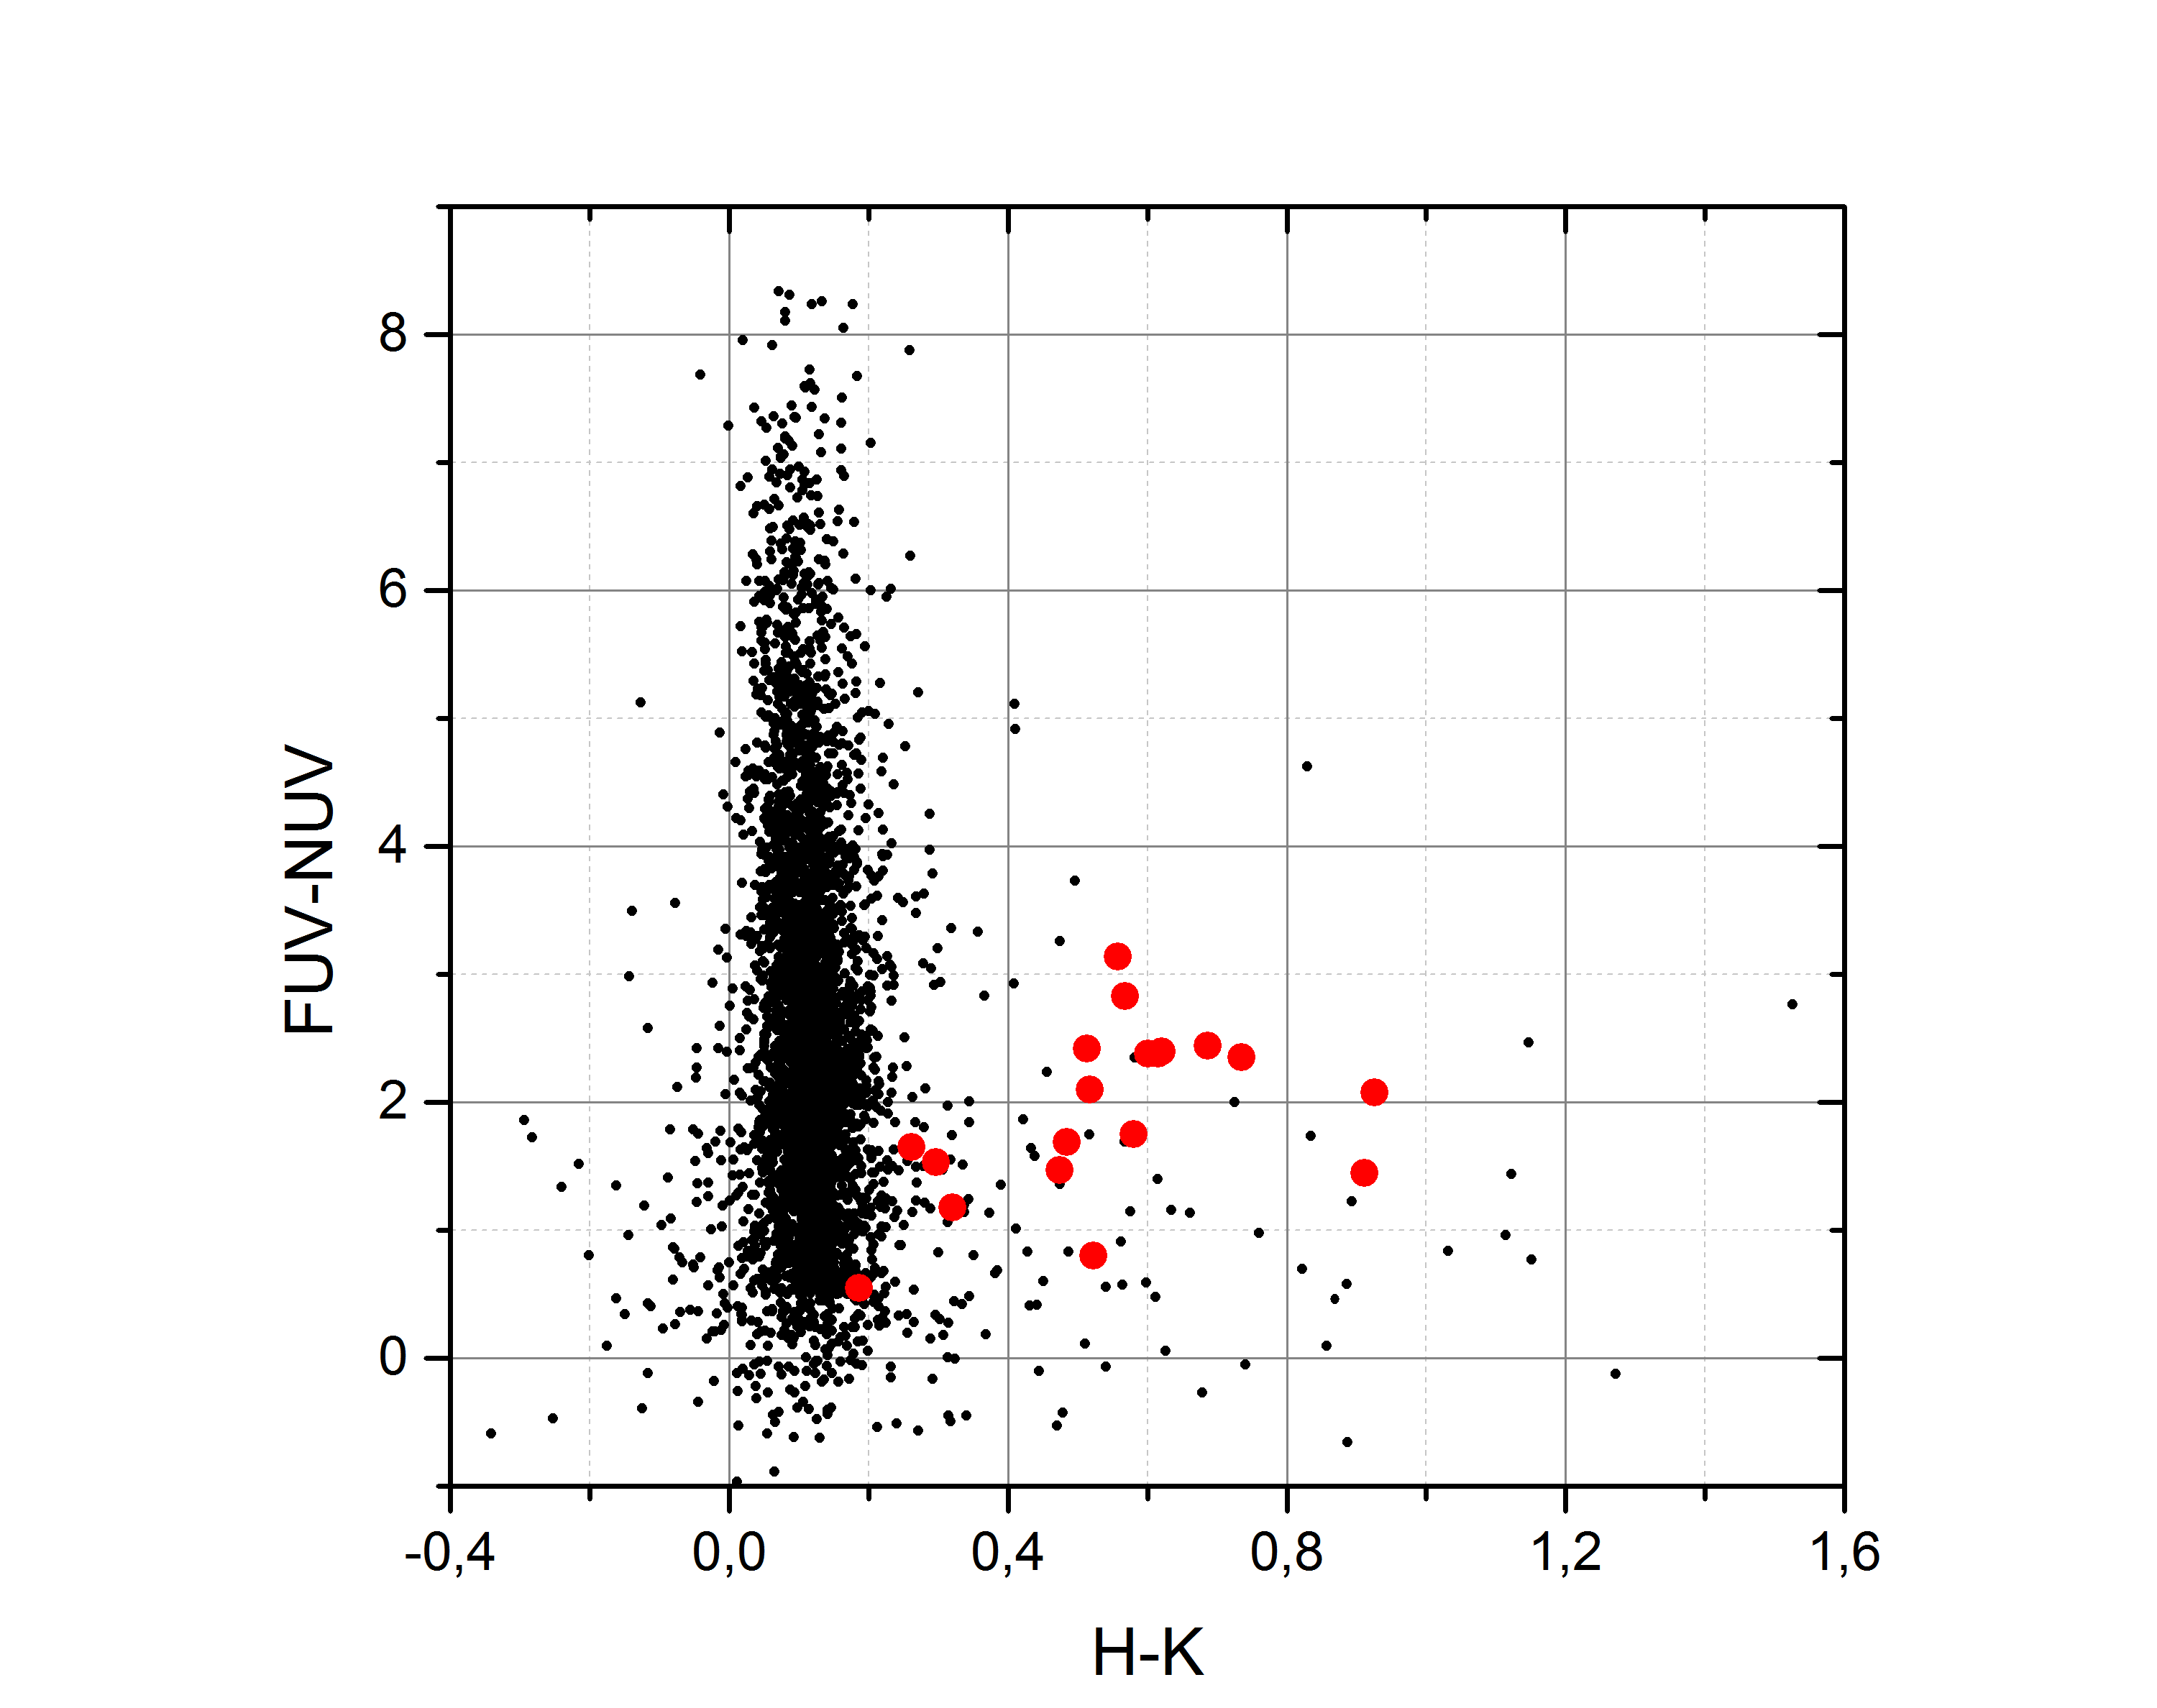
\includegraphics[width=1\linewidth]{Graph2.png} \\ FUV-NUV vs H-K}
\end{minipage}
\begin{minipage}[ht]{0.49\linewidth}
\center{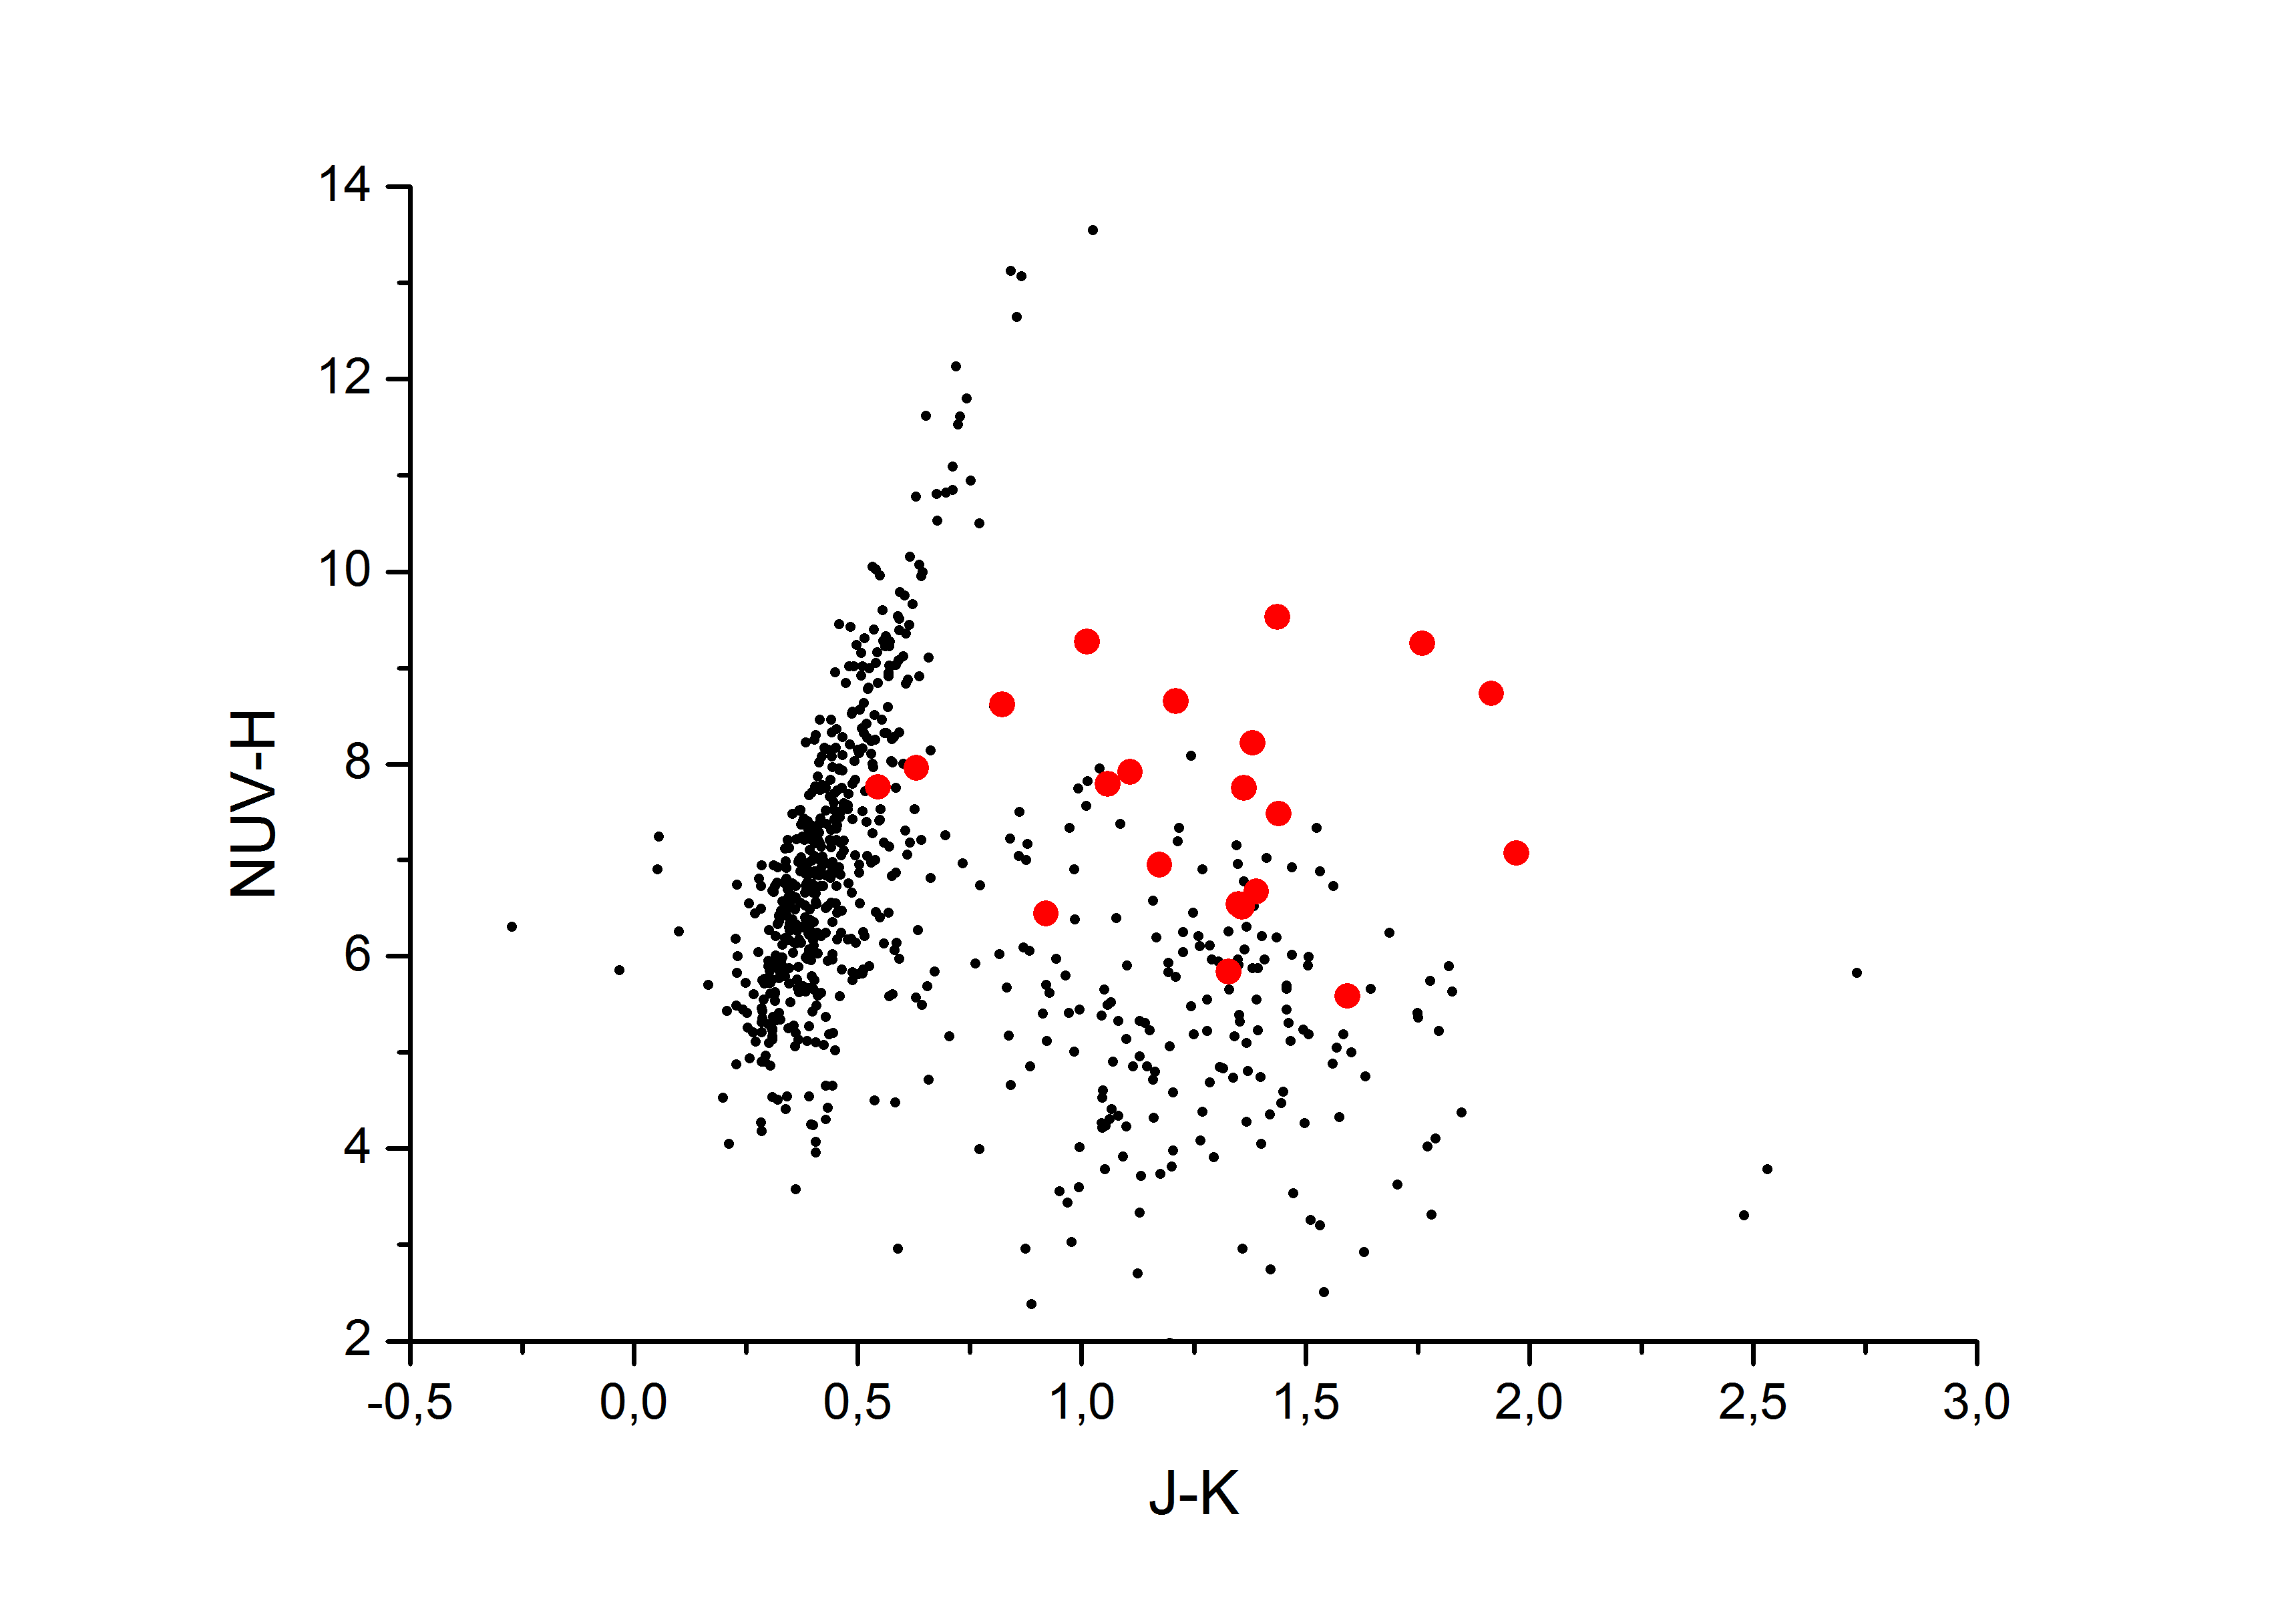
\includegraphics[width=1\linewidth]{Graph3.png} \\ NUV-H vs J-K}
\end{minipage}
\hfill
\begin{minipage}[ht]{0.49\linewidth}
\center{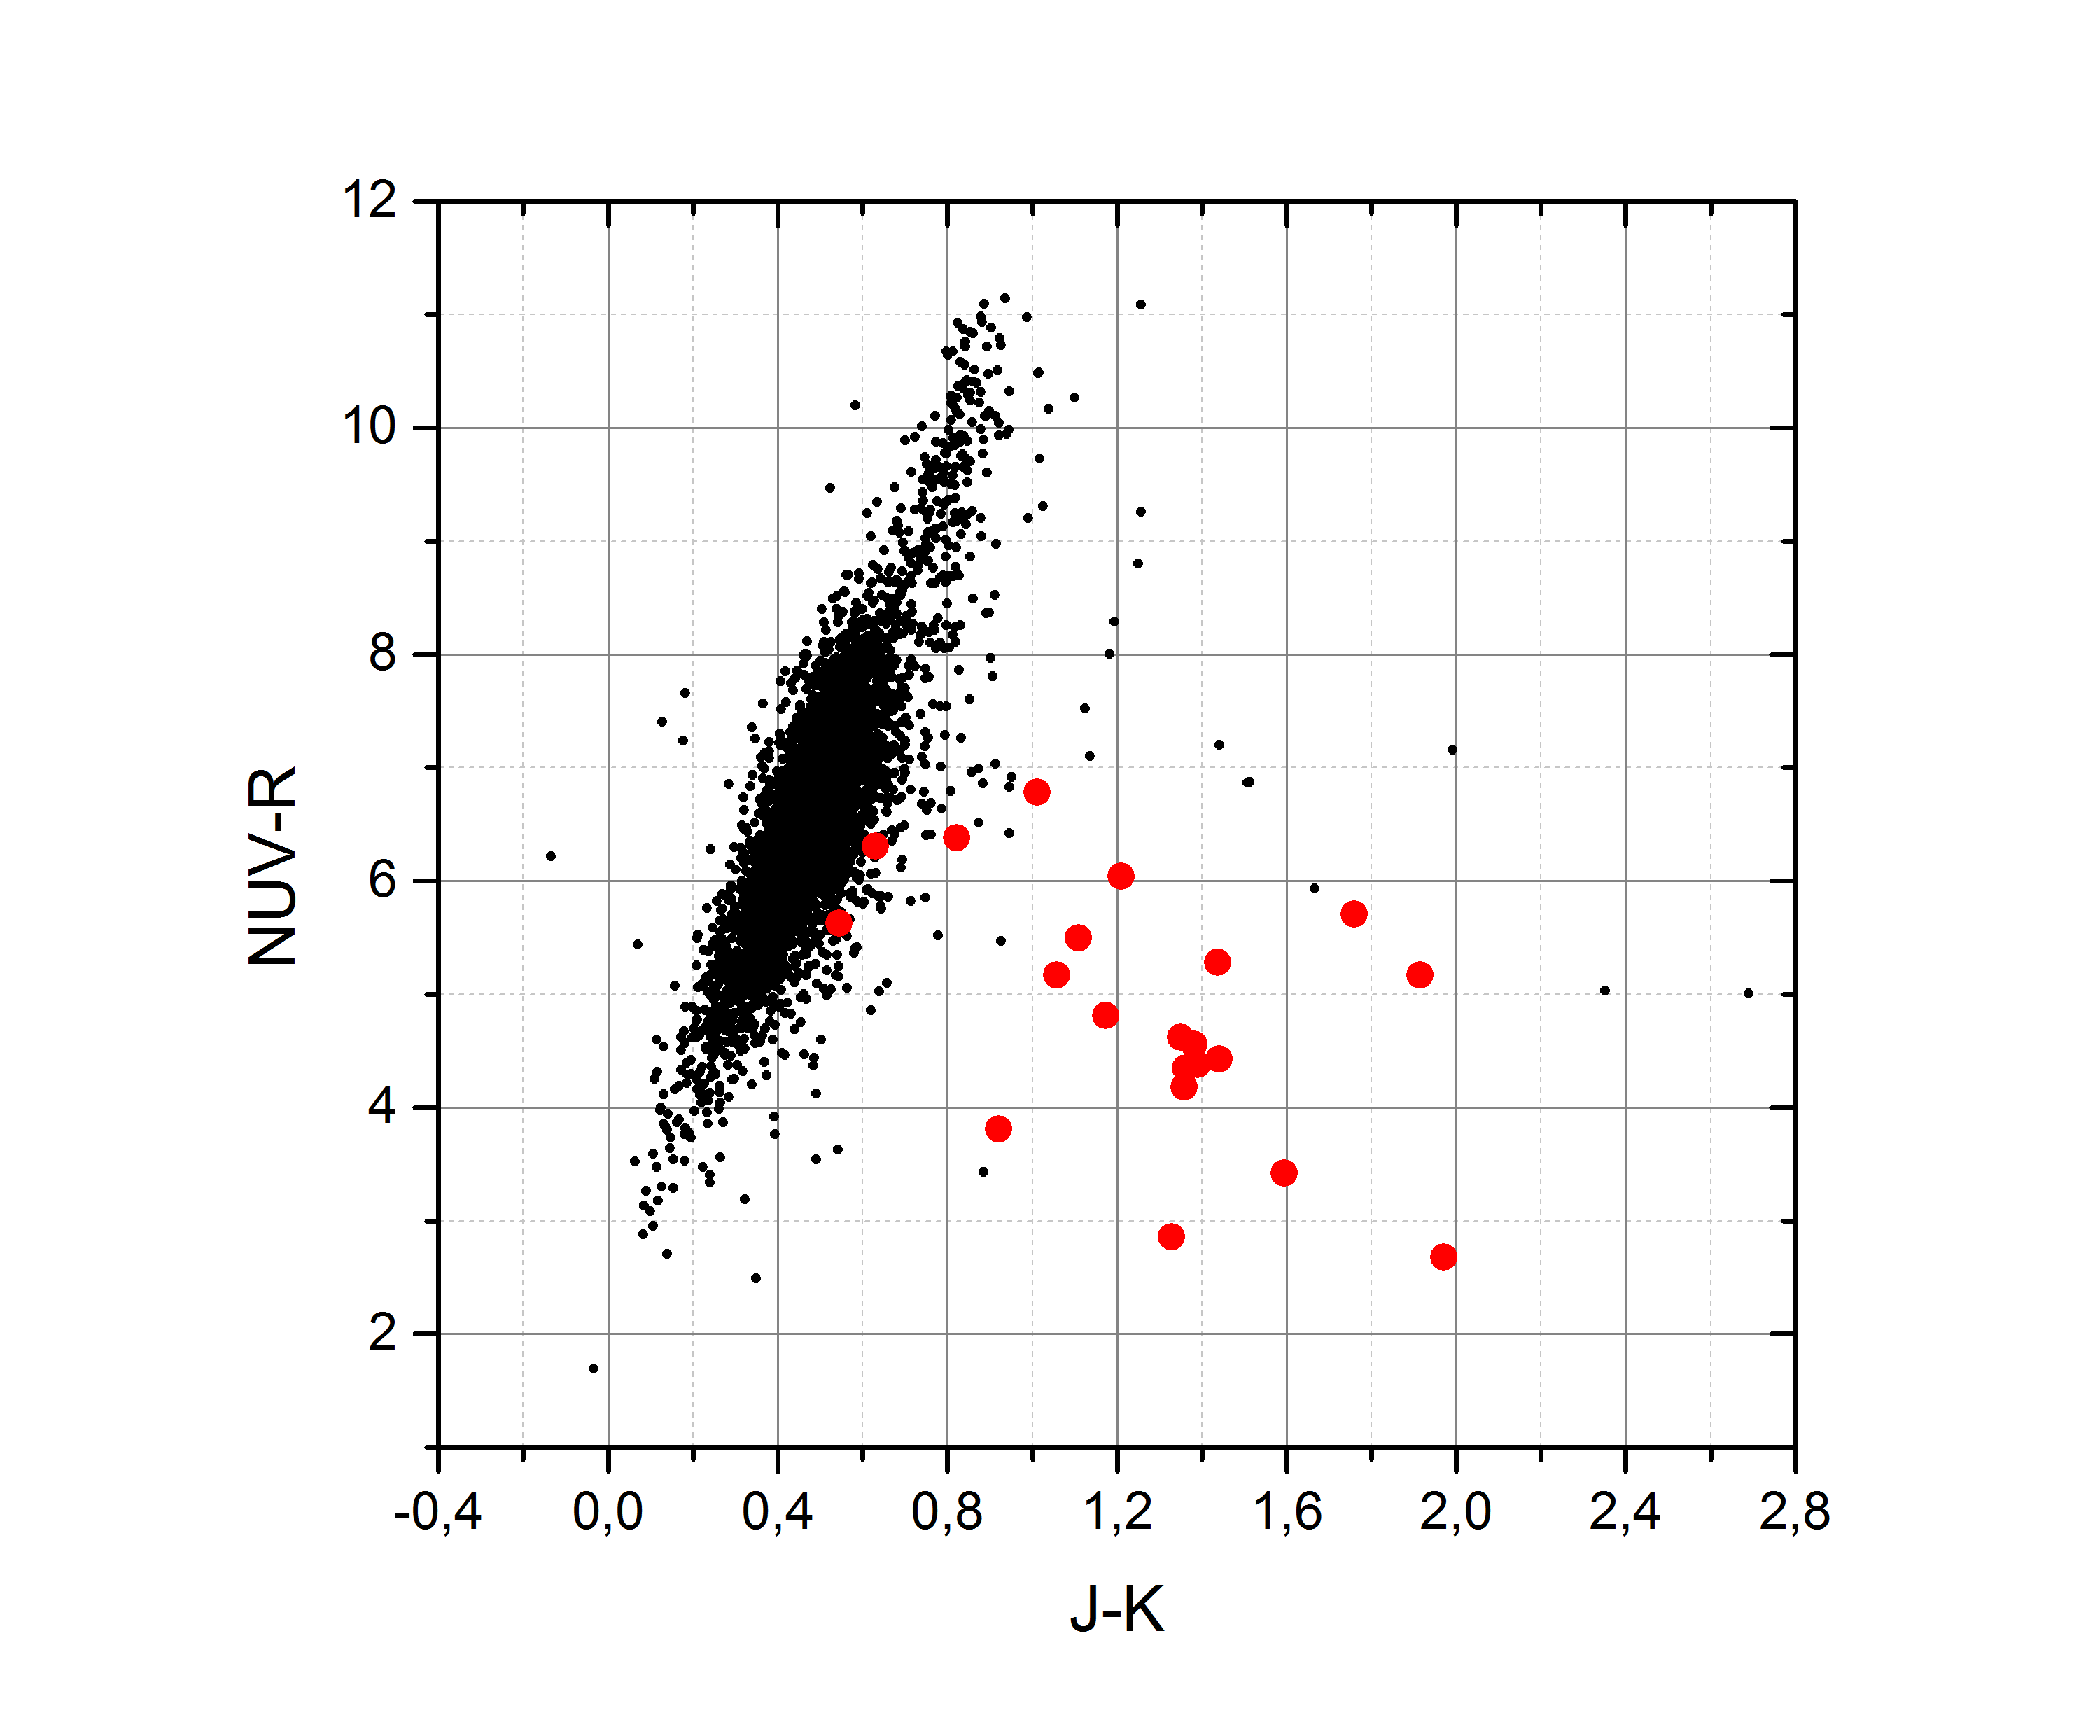
\includegraphics[width=1\linewidth]{Graph4.png} \\ NUV-R vs J-K}
\end{minipage}
\caption{Двухцветные диаграммы. Красным отмечены звёзды эталонной выборки}
\label{fig:colcol}
\end{figure}
Можно объяснить, почему для анализа выбраны именно диаграммы цвет-цвет. Потому что мы не можем сравнивать блеск разных звёзд, он зависит не только от типа звезды, но и от расстояния, поглощения. Нам нужно учесть избыток в инфракрасном диапазоне, поэтому по одной из осей откладывается разность двух ИК звёздных величин. Цвет по другой оси включает УФ величину.

На самом деле в работе \cite{AIGdC2014galex}  приводятся все типы диаграмм, которые мы можем построить, имея исходные данные. Однако именно на выбранных четырёх диаграммах звёзды типа Т Тельца лежат обособленно от остальных, как это видно из положения эталонной выборки.

Звёзды эталонной выборки выделены красным. Заметно, что они группируются в стороне от основной массы звёзд, относящихся к главной последовательности. Также можно видеть, что довольно много звёзд находятся в той же области диаграммы, что и эталоны.

На четвёртом графике рисунка \ref{fig:colcol} рядом с выборкой T Tauri звёзд почти нет других источников. Это связано с тем, что использующийся в данной диаграмме блеск в фильтре R измерен лишь для немногих звёзд в данной области -- тех, что присутствуют в каталоге UCAC4. 

\section{Критерии отбора}

В выборку включим все звёзды, положение которых на диаграммах близко к положению известных T Tauri. Для этого зададим границы, в которые должны входить цвета, причём все эталонные звёзды также должны попадать в эти границы.

На диаграмме NUV-H vs J-K эталонные T Tauri особенно сильно отделены от остальных звёзд. Это обусловлено тем, что в выборку IUE входят в основном яркие звёзды. К тому же большинство из них находится ближе, и как следствие меньше подвержено поглощению. Ниже группы эталонных звёзд на этой диаграмме находится много точек, у которых NUV-H меньше. Предполагая, что эти источники подверглись большему поглощению, то есть находятся глубже в молекулярном облаке, мы также включим их в список кандидатов, сдвинув границы по NUV-H в нижнюю сторону.

Диаграмма NUV-R от J-K должна дать нам не очень много кандидатов, однако её тоже нужно учесть. Как и NUV-H vs J-K, она даёт шанс неярким звёздам с неизмеренным FUV попасть в список кандидатов.

Теперь мы можем сформулировать критерии первичного отбора кандидатов:
\begin{itemize}
	\item FUV-NUV vs J-K: звёзды типа Т Тельца должны удовлетворять 0.5 < J - K < 2.4 и 0.4 < FUV - NUV < 4.6;
	\item	FUV-NUV vs H-K: звёзды типа Т Тельца должны удовлетворять 0.2 < H - K < 1.2 и 0.4 < FUV - NUV < 4.6;
	\item	NUV-H vs J-K: звёзды типа Т Тельца должны удовлетворять 0.5 < J - K < 2.4 и 4.2 < NUV - H < 11.0;
	\item	NUV-R vs J-K: звёзды типа Т Тельца должны удовлетворять 0.5 < J - K < 2.4 и 1.5 < NUV - R < 8.2;
\end{itemize}

Наша цель -- не только найти кандидаты в T Tauri звёзды, мы хотим, чтобы ни одна из них не была потеряна в ходе отбора, если это возможно. Поэтому на этом этапе мы оставляем те источники, которые удовлетворяют хотя бы одному из четырёх критериев.

Первые два критерия -- основные. Звёздные величины и цвета, входящие в них, соответствуют спектральным особенностям T Tauri звёзд, отличающих их от звёзд главной последовательности. Третий и четвёртый критерий тоже учитывают ультрафиолетовый избыток, так как в фильтр NUV попадают многие ключевые линии: (такие-то). Однако они подходят и для более слабых звёзд: тех, что находятся глубже в молекулярном облаке, чьё более коротковолновое излучение не дошло до нас из-за поглощения; для звёзд типа Т Тельца со слабыми линиями, у которых избыток настолько слаб, что не был зафиксирован детекторами GALEX.

\section{Результат и адекватность критериев}
После применения этих критериев к исходному списку мы получили следующие результаты.

Первому критерию удовлетворяет 164 источника, второму -- 100 источников, третьему -- 274, и четвёртому 94. В общий в список, включающий объединение этих четырёх, попало 302 источника.

Следует отметить, что последний критерий не добавляет ни одного нового источника в итоговый список, то есть нет кандидатов, удовлетворяющих одному лишь четвёртому критерию. Первые два критерия (основные) в сумме дают 215 источников. Оставшиеся 87 кандидатов попали в список по третьему критерию. Они могут не иметь FUV блеска.

Эффективность этих критериев может быть проверена по их способности детектировать все известные в изучаемой области звёзды типа Т Тельца. Но в туманности в созвездии Змея нет ни одной звезды, классифицированной как T Tauri, и ни одной, классифицированной как кандидат в T Tauri звёзды. Поэтому мы не можем проверить это напрямую.

Однако в работе \cite{AIGdC2014galex}, в которой аналогичные критерии применялись к звёздам в молекулярном облаке Тельца, эффективность критериев была проверена. Они оказались способны обнаружить все известные в TMC T Tauri звёзды, которых там насчитывается 31. 

Желание не упустить ни одну известную  звезду является одной из причин выбора более широких границ цвета при составлении критериев.



\chapter{Улучшение списка}
Теперь мы очистим список от источников, который могли попасть туда случайно. Это могут быть галактики, например, или горячие звёзды, потому что у них тоже присутствует избыток ультрафиолета.

\section{Удаление источников известного типа}
В первую очередь нужно очистить список от источников, которые заведомо не являются звёздами типа Т Тельца. Это могут быть галактики или звёзды, отношение которых к какому-то иному типу уже установлено.

С помощью сервиса Simbad можно узнать, чем является интересующий нас источник, имея лишь его координаты. Simbad (Set of Identifications, Measurements, and Bibliography for Astronomical Data ) -- это база данных об астрономических объектах, лежащих вне Солнечной системы \cite{wenger2000simbad}. Таким образом, загрузив в неё список координат возможных кандидатов, мы можем узнать их тип, если он когда-либо и кем-либо был определён.

Из 256 источников нашего списка Simbad идентифицировал лишь 43, причём 59 из них являются галактиками, и 15 -- звёздами. Галактики должны быть выброшены из списка. Почти все звёзды не отнесены ни к какому спектральному классу, поэтому их следует оставить. Две имеют класс G5, ещё две -- K2, одна -- K0 и является двойной. В соответствии с критериями принадлежности к типу Т Тельца, эти звёзды не удаляются из списка кандидатов.

Остальные источники не идентифицированы вовсе, то есть могут являться любым объектом. Они тоже, разумеется, должны быть оставлены в списке.

\section{Поиск галактик по собственным движениям}
Многие неидентифицированные Simbad источники могут также быть галактиками. Чтобы избавиться от них, мы можем сравнить их собственные движения. Те объекты, чьи собственные движения очень малы, то есть лежат в пределах погрешности наблюдений, с высокой вероятности лежат вне нашей Галактики.

Чтобы определить собственные движения, нужно заснять интересующую нас область и сравнить положения объектов с положениями, зафиксированными более ранними наблюдениями. Это может быть каталог DSS, который составлен на основе наблюдений, проведённых более 50 лет назад.

К сожалению, нам не удалось найти свежих фотографий неба в нужной области. 
В каталоге UCAC4 содержится информация о собственных движениях, но в него входят только объекты, заведомо являющиеся звёздами, поэтому он не может нам помочь.


\section{Оценка эффективных температур}
Некоторые попавшие в список источники могут иметь ультрафиолетовый избыток просто потому что у них очень большая температура. 

Для оценки эффективной температуры использовалась виртуальная обсерватория VOSA (Virtual Observatory SED Analyzer) \cite{bayo2008vosa}. Она позволяет построить распределение спектральной энергии (spectral energy distribution, SED) для источника, звёздные величины которого загружены пользователем, а также найти другую фотометрическую информацию об источнике с указанными координатами.

С помощью SED сервис может оценить чернотельную температуру источников, зная также расстояние до него и величину поглощения $A_v$. Расстояние до области нам известно, оно равно 415 пк [ссылка]. Поглощение, по оценкам, данным в работах [А И] и [другая], не превышает 0.3-0.5. Для оценки бралась величина $A_v=0.3$.

Согласно полученным оценкам, температуры кандидатов лежат в диапазоне от 3000 K до 9000 K. Отбросив все источники горячее 7000 K, сократим список ещё на 35 строк. После этого этапа в списке остаётся 208 кандидатов.




\chapter{Анализ}


\section{Диаграммы цвет-интенсивность}

Если построить диаграмму цвет-интенсивность \ref{fig:color-magnitude}, то можно увидеть, насколько отличается блеск кандидатов от блеска остальных источников в области и от эталонной выборки. Видно, что звёзды выборки гораздо ярче как кандидатов, так и всех звёзд области. 

Большинство кандидатов очень слабые, их звёздные величины находятся на грани чувствительности GALEX. Также видно, что цвет FUV-NUV у кандидатов может быть отрицательным, и также просто отличаться от эталонных. Это даёт представление о количестве кандидатов, пришедших в выборку с третьим, неультрафиолетовым критерием.

Источников на рисунке \ref{fig:color-magnitude} меньше, чем в итоговом списке, так как многие как кандидаты, так и остальные звёзды не имеют FUV измерений.

\begin{figure}[ht]
\center{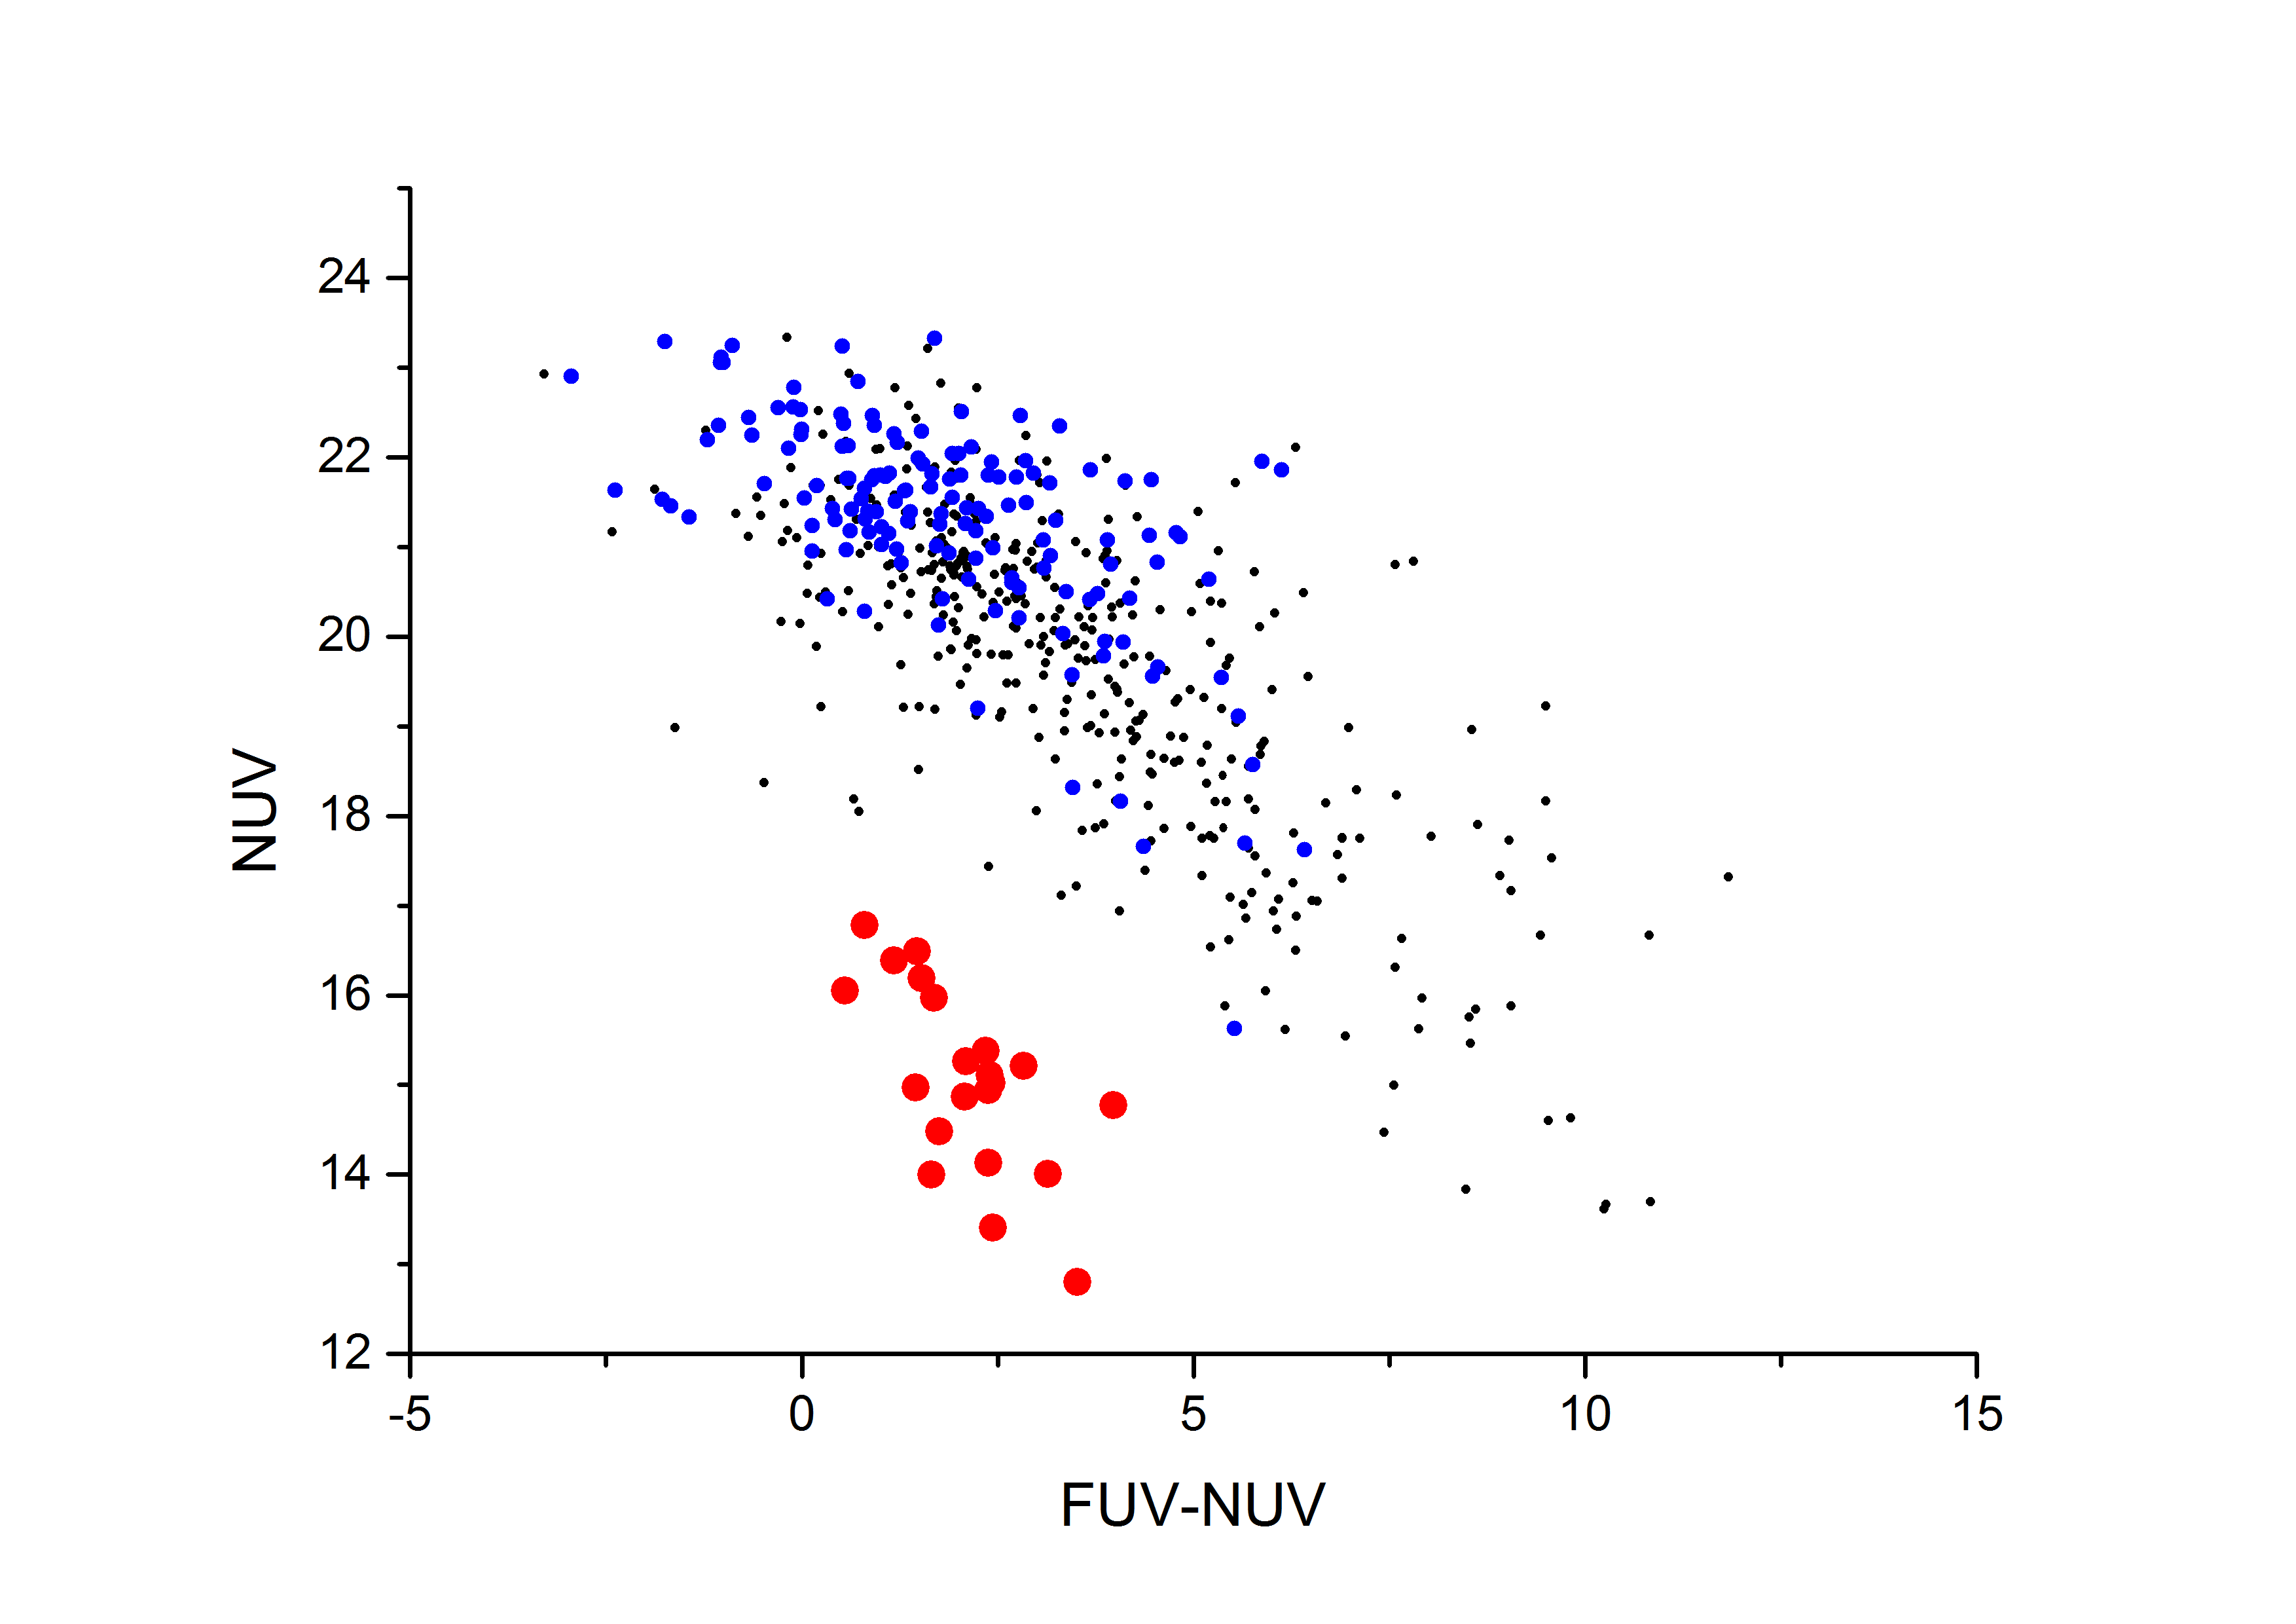
\includegraphics[width=0.6\linewidth]{colormagnitude.png}}
\hfill
\caption{Диаграмма цвет-интенсивность. Красным отмечены звёзды эталонной выборки, синим -- отобранные кандидаты}
\label{fig:color-magnitude}
\end{figure}

\section{Распределение спектральной энергии}

Сервис VOSA, использовавшийся для оценки эффективных температур, может строить распределение спектральной энергии, SED. Мы можем построить такую характеристику для эталонных звёзд, например, для T Tau, которая также входит в этот список, и сравнить с ней SED кандидатов. 

Как видно из рисунка, распределения не всегда похожи. Однако у большинства кандидатов в ультрафиолетовом диапазоне присутствует пик, подобный пику у T Tau.

\begin{figure}[ht]
\begin{minipage}[ht]{0.49\linewidth}
\center{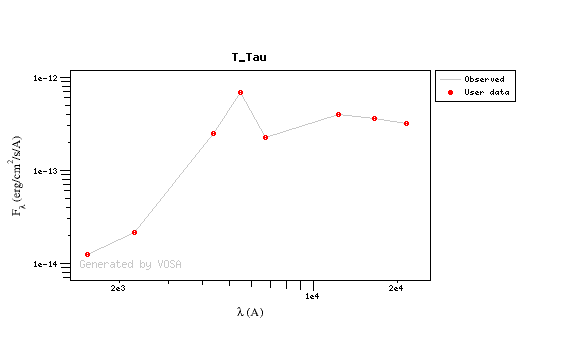
\includegraphics[width=1\linewidth]{T_Tau.png} \\ }
\end{minipage}
\hfill
\begin{minipage}[ht]{0.49\linewidth}
\center{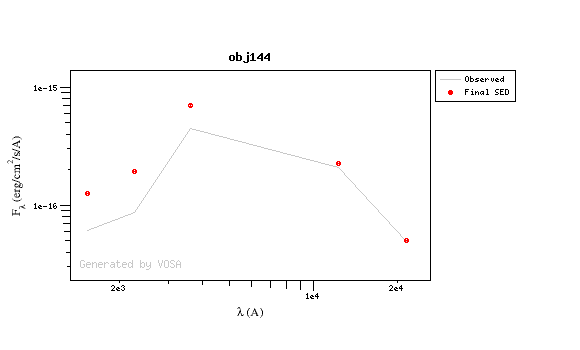
\includegraphics[width=1\linewidth]{obj144.png} \\ }
\end{minipage}
\begin{minipage}[ht]{0.49\linewidth}
\center{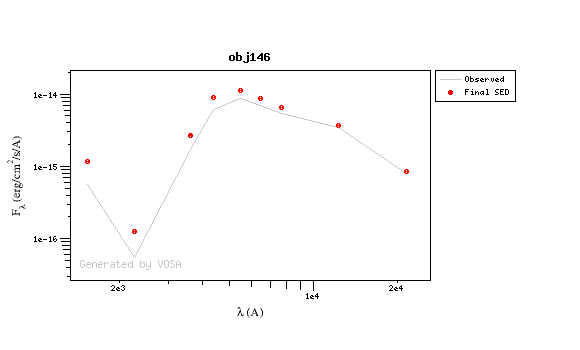
\includegraphics[width=1\linewidth]{obj146.png} \\ }
\end{minipage}
\hfill
\begin{minipage}[ht]{0.49\linewidth}
\center{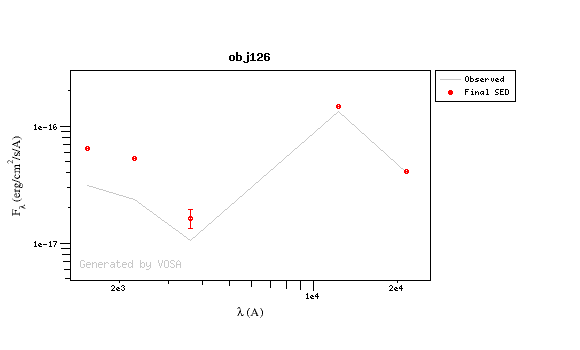
\includegraphics[width=1\linewidth]{obj126.png} \\ }
\end{minipage}
\caption{Распределение спектральной энергии (SED) для T Tau и некоторых из кандидатов}
\label{fig:sed}
\end{figure}

\section{Оценка поглощения}

Межзвёздное поглощение в исследуемой области определяется в основном наличием молекулярных облаков.
Так как ультрафиолет подвергается более сильному поглощению, чем ИК излучение, каталог GALEX содержит очень мало объектов в изучаемой части неба. Так как для звёзд Т Тельца характерен избыток УФ излучения, их видно значительно лучше, чем звёзды главной последовательности. Это может объяснить тот факт, что больше четверти первоначальных объектов попали в итоговый список кандидатов.

Наблюдения миссии GALEX относятся только к периферии облаков, где поглощение значительно ниже. По некоторым оценкам, его величина $A_v < 0.5$ \cite{AIGdC2014galex} по другим $A_v < 0.5$ \cite{park2012far}, и таким поглощением можно пренебречь.

Значение $A_v = 0.3$ использовалось для оценки эффективных температур. Также оно учитывалось при построении SED. Но существенного влияния по сравнению с $A_v = 0$ замечено не было.

\section{Расположение}
Картинки с координатами и собственными движениями.

\section{Классические и со слабыми линиями}
В соответствии с результатами, полученными в аналогичном исследовании \cite{AIGdC2014galex}, WTTS и CTTS также находятся в разных областях двухцветной диаграммы FUV-NUV vs J-K:
\begin{itemize}
	\item Положение WTTS определяется линией $FUV - NUV = -(3.88 \pm 0.61)(J - K) + (5.64 \pm 0.55)$, среднеквадратичное отклонение равно 0.59.
	\item CTTS имеют нормальное распределение по оси $J - K$ со средним значением $a = 1.4$ и дисперсией $\sigma = 0.4$. По оси $FUV - NUV$ они распределены равномерно.
\end{itemize}

\begin{figure}[ht]
\center{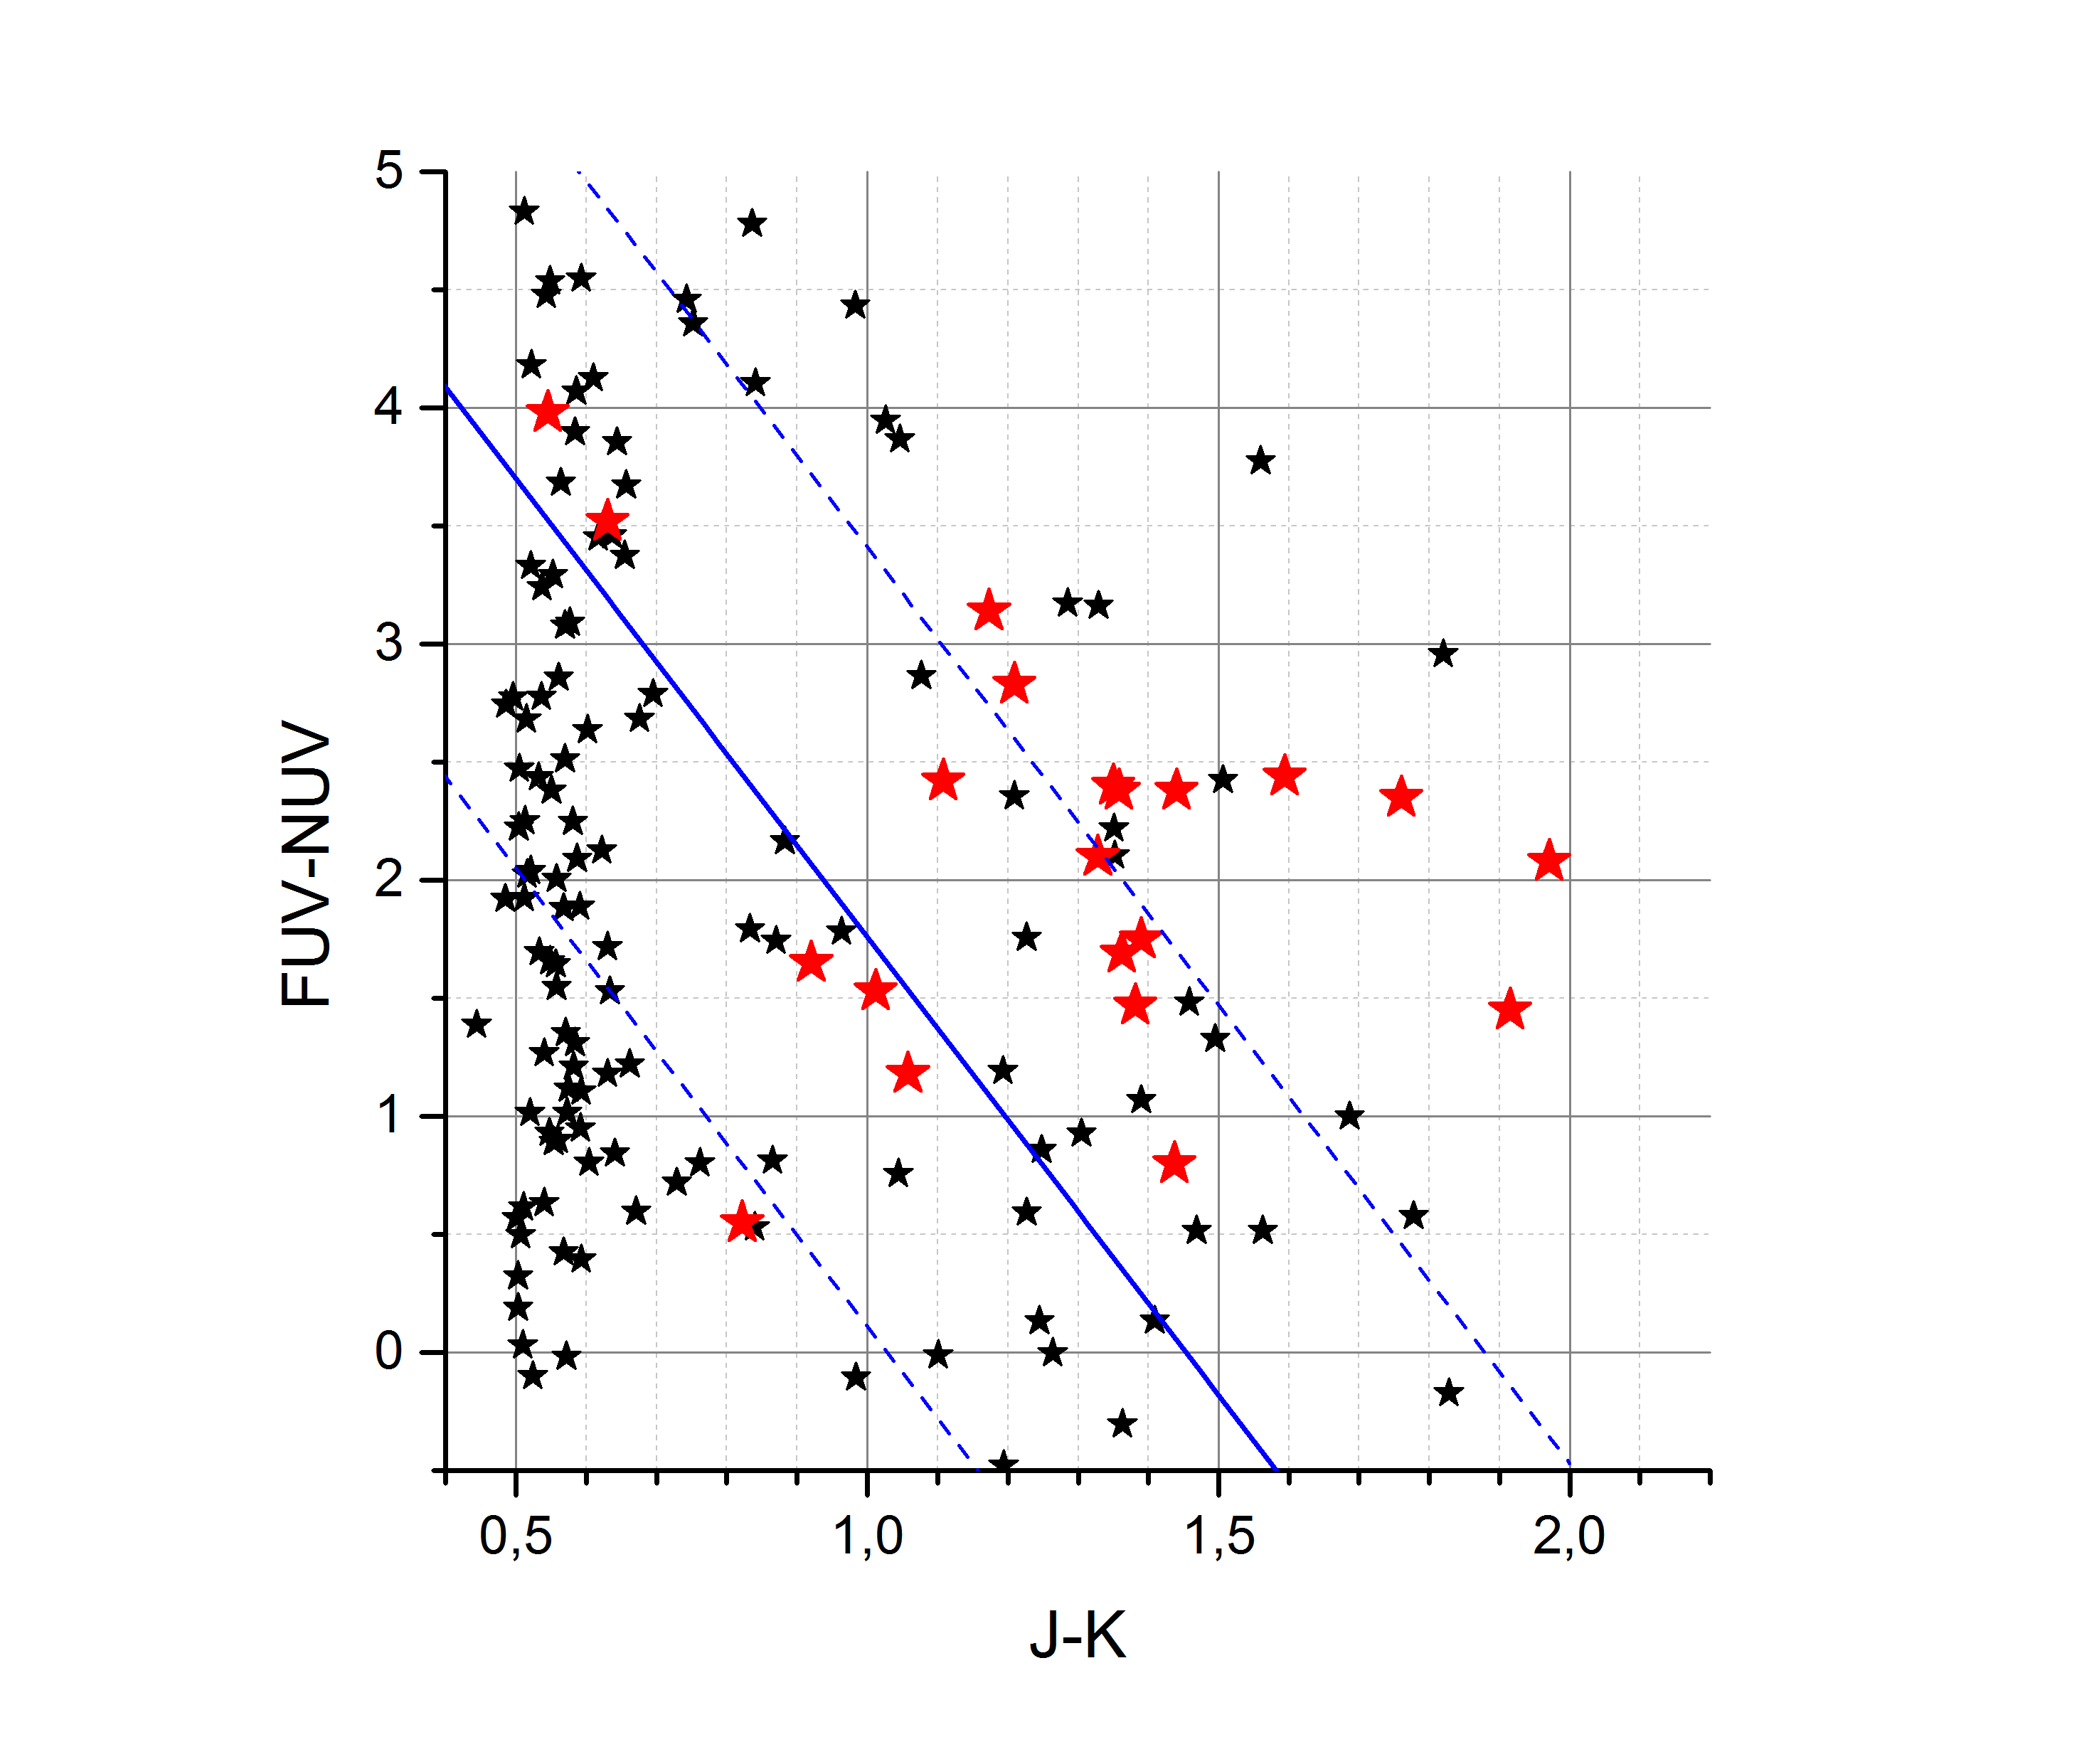
\includegraphics[width=0.6\linewidth]{trend.png}}
\hfill
\caption{Двухцветная диаграмма FUV - NUV vs J - K. Красным обозначены звёзды эталонной выборки, чёрным -- кандидаты. Синими прямыми выделена область, в которой расположены WTTS.}
\label{fig:trend}
\end{figure}

Теперь можно распределить кандидаты в группы согласно этим результатам. К звёздам типа Т Тельца со слабыми линиями относим те, что лежат между штриховыми прямыми на рисунке \ref{fig:trend} (границы взяты втрое шире, чем коридор ошибок приближения), и имеют FUV~-~NUV > 3.5. К классическим T Tauri отнесём источники, у которых 0 < FUV~-~NUV < 3.5. Остальные кандидаты, включая не имеющие FUV, будем считать кандидатами в T Tauri звёзды без более детальной классификации.





\chapter{Выводы}
Итак, мы получили финальный список кандидатов в звёзды типа Т Тельца, всего их целых N штук.

Мы сделали всё, что мы сделали, мы молодцы. 

Теперь можно понаблюдать все кандидаты со Спектра-УФ, чтобы выяснить, действительно ли они типа T Tauri. Но можно и улучшить список ещё, если очень хочется, а именно -- пронаблюдать эти источники на БТА и уточнить их звёздные величины в видимом диапазоне.

Спасибо мама, папе, Ленке, Вове, Лохматому и Булке за моральную поддержку и веру в меня, спасибо спасибо.






\addcontentsline{toc}{chapter}{Список литературы}
\bibliography{Bib}     %% имя библиографической базы (bib-файла) 

\end{document}
